% A (minimal) template for problem sets and solutions using the exam document class

% Organization:
%% Define new commands, macros, etc. in macros.tex
%% Anything that you would put before \begin{document} should go in prelude.tex

%% For multiple psets, each should get its own file to \input into main with a \section{}

\documentclass[answers]{exam}
\usepackage{amsmath}
\setcounter{MaxMatrixCols}{20} % since previously max cols of bmatrix is only 10
\usepackage{amsthm}
\usepackage{amsfonts}
\usepackage{amssymb}
\usepackage{mathrsfs}
\usepackage[autostyle]{csquotes}
\renewcommand{\qedsymbol}{$\blacksquare$}

\usepackage{fullpage}
\usepackage[top=2cm, bottom=4.5cm, left=2.5cm, right=2.5cm]{geometry}
\usepackage{amsmath,amsthm,amsfonts,amssymb,amscd}
\usepackage{lastpage}
\usepackage{enumerate}
\usepackage{fancyhdr}
\usepackage{mathrsfs}
\usepackage{xcolor}
\usepackage{graphicx}
\usepackage{listings}
\usepackage{hyperref}
\usepackage{listings}
\usepackage{float}  % for fixed figure
\usepackage[framed,numbered,autolinebreaks,useliterate]{mcode} % for matlab code
\hypersetup{%
  colorlinks=true,
  linkcolor=blue,
  linkbordercolor={0 0 1}
}
\graphicspath{ {./images/} }

\renewcommand\lstlistingname{Algorithm}
\renewcommand\lstlistlistingname{Algorithms}
\def\lstlistingautorefname{Alg.}

\lstdefinestyle{Python}{
    language        = Python,
    frame           = lines, 
    basicstyle      = \footnotesize,
    keywordstyle    = \color{blue},
    stringstyle     = \color{green},
    commentstyle    = \color{red}\ttfamily
}

\setlength{\parindent}{2em}
\setlength{\parskip}{0.05in}

% Edit these as appropriate
\newcommand\course{EE4212 Computer Vision}
\newcommand\hwnumber{}                  % <-- homework number
\newcommand\NetIDa{github}           % <-- NetID of person #1
\newcommand\NetIDb{lkevinzc}           % <-- NetID of person #2 (Comment this line out for problem sets)

\pagestyle{fancyplain}
\headheight 35pt
\lhead{\NetIDa}
\lhead{\NetIDa\\\NetIDb}                 % <-- Comment this line out for problem sets (make sure you are person #1)
\chead{\textbf{\Large Assignment 1 \hwnumber}}
\rhead{\course \\ \today}
\lfoot{}
\cfoot{}
\rfoot{\small\thepage}
\headsep 1.5em

\begin{document}

%% \union - Example: \union{j \in J}{A_j}
\newcommand{\union}[2]{\underset{#1}\bigcup #2}

%% \inter - like \union, but with \bigcap
\newcommand{\inter}[2]{\underset{#1}\bigcap #2}

%% change solution title from "solution" to "answer"
\renewcommand{\solutiontitle}{\noindent\textbf{Answer:}\par\noindent}

%% Content goes here


\section{Projection Model, Homogeneous coordinates}
\begin{questions}
\question
\begin{parts}
% question 1a
\part
* Suppose you have two parallel lines in 3-D space, one passing through the point$ (100,100,1000)$, the other through $(200,200,1100)$. The lines are parallel to the vector $(1,2,1)$. The lines are observed by a unit focal length camera at the origin (i.e. the camera reference frame and the world reference frame are identical). All coordinates are in camera coordinates. What is their point of intersection in the image? (Hint: the point of infinity along $\ell_i$ in 3-D space is given by $\lim_{\lambda_i\to\infty} \ell_i = \left(\begin{array}{c}X_i \\ Y_i \\ Z_i \\ \end{array} \right) + \lambda_i \left(\begin{array}{c}a \\ b \\ c \\ \end{array} \right)$, where $\left(\begin{array}{c}X_i \\ Y_i \\ Z_i \\ \end{array} \right)$ and $\left(\begin{array}{c}a \\ b \\ c \\ \end{array} \right)$ are a point on the line and its direction respectively)


\begin{solution}
  Denote the two parallel lines as follows:
  \[ \ell_a = \left(\begin{array}{c}100 \\ 100 \\ 1000 \\ \end{array} \right) + \lambda_a\left(\begin{array}{c}1 \\ 2 \\ 1 \\ \end{array} \right), \ell_b = \left(\begin{array}{c}200 \\ 200 \\ 1100 \\ \end{array} \right) + \lambda_b\left(\begin{array}{c}1 \\ 2 \\ 1 \\ \end{array} \right) \]
  
  Set $\lambda_a=100$ and $\lambda_a=200$ respectively to get two points on $\ell_a$:
  \[ P_{1a} = \left(\begin{array}{c}200 \\ 300 \\ 1100 \\ \end{array} \right), P_{2a} = \left(\begin{array}{c}300 \\ 500 \\ 1200 \\ \end{array} \right) \]
  
  Using the linear mapping of the perspective projection:
  
  \begin{equation}
  \left( \begin{array} { l } { x } \\ { y } \\ { w } \end{array} \right) = \left[ \begin{array} { c c c c } { f } & { 0 } & { 0 } & { 0 } \\ { 0 } & { f } & { 0 } & { 0 } \\ { 0 } & { 0 } & { 1 } & { 0 } \end{array} \right] \left( \begin{array} { c } { X _ { c } } \\ { Y _ { c } } \\ { Z _ { c } } \\ { 1 } \end{array} \right)
  \end{equation}
  
  The corresponding points (in $\mathcal{P}^2$) of $\mathbf{P}_{1a}$ and $\mathbf{P}_{2a}$ on the image are:
  \[ P^{'}_{1a} = \left[ \begin{array} { c c c c } { 1 } & { 0 } & { 0 } & { 0 } \\ { 0 } & { 1 } & { 0 } & { 0 } \\ { 0 } & { 0 } & { 1 } & { 0 } \end{array} \right] \left( \begin{array} { c } { 200 } \\ { 300 } \\ { 1100 } \\ { 1 } \end{array} \right) = \left(\begin{array}{c}200 \\ 300 \\ 1100 \\ \end{array} \right) \]
  
  \[ P^{'}_{2a} = \left[ \begin{array} { c c c c } { 1 } & { 0 } & { 0 } & { 0 } \\ { 0 } & { 1 } & { 0 } & { 0 } \\ { 0 } & { 0 } & { 1 } & { 0 } \end{array} \right] \left( \begin{array} { c } { 300 } \\ { 500 } \\ { 1200 } \\ { 1 } \end{array} \right) = \left(\begin{array}{c}300 \\ 500 \\ 1200 \\ \end{array} \right) \]
  
  The corresponding line (in $\mathcal{P}^2$) of $\ell_{a}$ on the image are formed by two points above:
  \[ \ell^{'}_a = P^{'}_{1a} \times P^{'}_{2a} = \left(\begin{array}{c}-190000 \\ 90000 \\ 10000 \\ \end{array} \right) \]
  
  Similarly, the corresponding line (in $\mathcal{P}^2$) of $\ell_{b}$ on the image can be obtained:
  \[ \ell^{'}_b = \left(\begin{array}{c}-200000 \\ 90000 \\ 20000 \\ \end{array} \right) \]
  
  Therefore, the intersection point (in $\mathcal{P}^2$) of the two parallel lines (in $\mathcal{N}^{3}$) on the image is:
  \[ P = \ell^{'}_a \times \ell^{'}_b  = \left(\begin{array}{c} 9 \times 10^{8} \\ 1.8 \times 10^{9} \\ 9 \times 10^{8} \\ \end{array} \right) \]
  
  Converting back to $\mathcal{N}^{2}$, $P = \left(\begin{array}{c} 1 \\ 2 \\ \end{array} \right)$ is the intersection point on the image.
  
\end{solution}

% question 1b
\part
Given the 3D coordinates of several corresponding points $P_i$ and $P_{i}^{'}$ in two views, you are required to find the 3D rotation $\mathbf{R}$ and translation $\mathbf{T}$ that relate the two views ($P_{i}^{'} = \mathbf{R}P_{i} + \mathbf{T}$). Formulate a linear least squares algorithm (of the form $\mathbf{A} \mathbf{x} = \mathbf{b}$) that ignores the orthogonality constraint associated with $\mathbf{R}$ (that is, it is okay if the solution for $\mathbf{R}$ returned by your formulation is not orthogonal). State the entries of the matrix $\mathbf{A}$, and the vectors $\mathbf{x}$ and $\mathbf{b}$.

\begin{solution}
    Denote $P_{i} = \left( \begin{array} {c} {x_{i}} \\ {y_{i}} \\{z_{i}} \\ \end{array}\right)$, $P_{i}^{'} = \left( \begin{array} {c} {x^{'}_{i}} \\ {y^{'}_{i}} \\{z^{'}_{i}} \\ \end{array}\right)$, $\mathbf{R} = \left[ \begin{array} {c c c} {R_{11}} & {R_{12}} & {R_{13}} \\ {R_{21}} & {R_{22}} & {R_{23}} \\ {R_{31}} & {R_{32}} & {R_{33}} \\ \end{array} \right]$, $\mathbf{T} = \left(\begin{array}{c} t_{1} \\ t_{2} \\ t_{3} \\ \end{array} \right)$.
    
    The relationship between points in two views is determined by $P_{i}^{'} = \mathbf{R}P_{i} + \mathbf{T}$, which can also be written as a linear mapping in the homogeneous coordinate: 
    \begin{equation}
        \begin{split}
            \left(\begin{array}{c}x_{i}^{'} \\ y_{i}^{'} \\ z_{i}^{'} \\ 1 \\ \end{array} \right) 
            & = \left[ \begin{array} { c c } { \mathbf{R} } & \mathbf{T}  \\ { \mathbf{0}^{T} } & { 1 }  \end{array} \right] \left(\begin{array}{c}x_{i} \\ y_{i} \\ z_{i} \\ 1 \\ \end{array} \right)\\
            & = \left[ \begin{array} { c c c c } {R_{11}} & {R_{12}} & {R_{13}} & { t_{1} } \\ {R_{21}} & {R_{22}} & {R_{23}} & { t_{2} } \\ {R_{31}} & {R_{32}} & {R_{33}} & { t_{3} } \\ {0} & {0} & {0} & {1} \end{array} \right] \left(\begin{array}{c}x_{i} \\ y_{i} \\ z_{i} \\ 1 \\ \end{array} \right)
        \end{split}
    \end{equation}
    
    Expanding Eq. (2), three independent equations can be obtained:
    \[x_{i}^{'} = R_{11} x_{i} + R_{12} y_{i} + R_{13} z_{i} + t_{1} + \cdots,\]
    \[y_{i}^{'} = R_{21} x_{i} + R_{22} y_{i} + R_{23} z_{i} + t_{2} + \cdots,\]
    \[z_{i}^{'} = R_{31} x_{i} + R_{32} y_{i} + R_{33} z_{i} + t_{3} + \cdots,\]
    where \enquote{$\cdots$} means padding zeros to complete the expressions of the form $r^{T} x \in \mathcal{R}$ ($r, x \in \mathcal{R}^{12}$).
    
    Hence, in the linear least squares formulation, the unknown $\mathbf{x}=\left( \begin{array} {c} {R_{11}} \\ {R_{12}} \\ {R_{13}} \\ {R_{21}} \\ \vdots \\ {R_{33}} \\ {t_1} \\ {t_2} \\ {t_3} \\ \end{array} \right) \in \mathcal{R}^{12}$.
    
    There are three equations to impose constraints to solve for different parts of entries of $\mathbf{x}$:
    \[ \mathbf{A}_{1} \mathbf{x} = \mathbf{b}_{1}, \ \mathbf{A}_{2} \mathbf{x} = \mathbf{b}_{2},\ \mathbf{A}_{3} \mathbf{x} = \mathbf{b}_{3}, \ \text{where}\]
    \[ \mathbf{A}_{1} = \begin{bmatrix}
        \vert & \vert & \vert & \vert &        & \vert & \vert & \vert & \vert\\
        x_{i} & y_{i} & z_{i} & 0     & \cdots & 0     & 1     & 0     & 0    \\
        \vert & \vert & \vert & \vert &        & \vert & \vert & \vert & \vert\\
    \end{bmatrix}, \ \mathbf{b}_{1} = \left( \begin{array} {c} \vert \\ x_{i}^{'} \\ \vert \\ \end{array} \right) \]
    
    \[ \mathbf{A}_{2} = \begin{bmatrix}
    \vert&\vert&\vert&\vert&\vert&\vert&\vert&&\vert&\vert&\vert\\
    0&0&0& x_{i} & y_{i}  & z_{i} & 0   & \cdots & 0   & 1 & 0\\
    \vert&\vert&\vert&\vert&\vert&\vert&\vert&&\vert&\vert&\vert\\
    \end{bmatrix}, \ \mathbf{b}_{2} = \left( \begin{array} {c} \vert \\ y_{i}^{'} \\ \vert \\ \end{array} \right) \]
    
    \[ \mathbf{A}_{3} = \begin{bmatrix}
    \vert &  & \vert & \vert &\vert  & \vert & \vert & \vert & \vert\\
    0 & \cdots & 0 & x_{i} & y_{i} & z_{i} & 0     & 0 & 1    \\
    \vert &  & \vert & \vert &\vert  & \vert & \vert & \vert & \vert\\
    \end{bmatrix}, \ \mathbf{b}_{3} = \left( \begin{array} {c} \vert \\ z_{i}^{'} \\ \vert \\ \end{array} \right) \]
    
    To be more compact, we could also write them as one equation:
    \[ \mathbf{A} \mathbf{x} = \mathbf{b}, \ \text{where} \]
    \[ \mathbf{A} = \begin{bmatrix}
        \vdots & \vdots & \vdots & \vdots & \vdots & \vdots & \vdots & \vdots & \vdots& \vdots& \vdots& \vdots\\
        x_{i} & y_{i} & z_{i} & 0& 0& 0& 0& 0&  0     & 1     & 0     & 0    \\
        \vdots & \vdots & \vdots & \vdots & \vdots & \vdots & \vdots & \vdots & \vdots& \vdots& \vdots& \vdots\\
        
        \vdots & \vdots & \vdots & \vdots & \vdots & \vdots & \vdots & \vdots & \vdots& \vdots& \vdots& \vdots\\
        0& 0& 0& x_{i} & y_{i} & z_{i} &  0& 0&  0     & 0     & 1     & 0    \\
        \vdots & \vdots & \vdots & \vdots & \vdots & \vdots & \vdots & \vdots & \vdots& \vdots& \vdots& \vdots\\
        
        \vdots & \vdots & \vdots & \vdots & \vdots & \vdots & \vdots & \vdots & \vdots& \vdots& \vdots& \vdots\\
        0& 0& 0& 0& 0&  0&x_{i} & y_{i} & z_{i} &  0     & 0     & 1    \\
        \vdots & \vdots & \vdots & \vdots & \vdots & \vdots & \vdots & \vdots & \vdots& \vdots& \vdots& \vdots\\
    \end{bmatrix}, \ \mathbf{b} = \left( \begin{array} {c} \vdots \\ x_{i}^{'} \\ \vdots \\ \vdots \\ y_{i}^{'} \\ \vdots \\ \vdots \\ z_{i}^{'} \\ \vdots \\ \end{array} \right)\]
\end{solution}

% question 1c
\part
You are now given two sets of corresponding point clouds $P_{i}$ and $P_{i}^{'}$, in the files \texttt{pts.txt} and \texttt{pts\_prime.txt} respectively. Each row is a 3D coordinate, possibly contaminated with some noise. Write a Matlab routine to estimate the optimal values of $\mathbf{R}$ and $\mathbf{T}$ in the least squares sense via SVD, using the formulation in (b). Compute the determinant of $\mathbf{R}$ using the Matlab function \enquote{det}, and comment on the resulting values.

\begin{solution}
    My Matlab commands run as follows:
    \begin{lstlisting}
P = importdata('pts.txt');
P_prime = importdata('pts_prime.txt');
pad = zeros([200, 3]);
A = [P;pad;pad];
A = [A [pad;P;pad]];
A = [A [pad;pad;P]];
last_cols = [ones([200,1]) zeros([200,1]) zeros([200,1]); [zeros([200,1]) ones([200,1]) zeros([200,1])]; [zeros([200,1]) zeros([200,1]) ones([200,1])]];
A = [A last_cols];
b = [P_prime(:,1); P_prime(:,2); P_prime(:,3)];
[U,S,V]=svd(A);
s=diag(S);
disp('singular values:'), disp(s')
bt=U'*b;
y=bt(1:12)./s;
x=V*y;
disp('x using SVD, all singular values:'), disp(x')
disp('||Ax-b||:'), disp(norm(A*x-b))
R = reshape(x(1:9), [3,3])';
det(R)
    \end{lstlisting}
    For the results, the unknown is solved to be:
    \[
    \begin{split}
    x ^ {T} = (0.9782, -0.0084,0.0094 
            &,0.0202, -0.0046,0.9979,-0.0016, \\
            &-0.9940,-0.0007,-0.0365,-4.0009,4.0021)
    \end{split}
    \] 
    using SVD in Matlab. And the residual $||Ax-b|| = 3.5757$. The rotation matrix 
    \[
    R = \begin{bmatrix} 
        0.9782  & -0.0084   &  0.0094  \\
        0.0202 & -0.0046 &  0.9979  \\ 
         -0.0016 & -0.9940  &   -0.0007 \\
    \end{bmatrix}\] 
    The determinant $det(R)=0.9701$, which is close to 1, showing that the resulted rotation matrix is reasonable since it should not change rigid body's volume. However, as we can see it is a bit off due to som noises.
\end{solution}

% question 1d
\part
If the world homogeneous coordinates are $(X_w, Y_w, Z_w, W_w)$, the image plane homogeneous coordinates are $(u, v, w)$, and they are related by: $\left( \begin{array} { c } { u } \\ { v } \\ { w } \end{array} \right) \sim M \left( \begin{array} { c } { X _ { w } } \\ { Y _ { w } } \\ { Z _ { w } } \\ { W _ { w } } \end{array} \right)$.
\begin{subparts}
    \subpart
    Find the $3 \times 4$ matrix M as a function of $\alpha$, $h$, according to Figure 1 below (in the left diagram, the axis $X$ and $X_w$ are pointing directly out of the paper). Assume that the only intrinsic camera parameter is the focal length $f$ (given in pixel unit). Use $P_c = RP_w +t$ to relate the camera coordinates $P_c$ and the world coordinates $P_w$. $R$ is the orientation of the world with respect to the camera; $t$ is the world origin expressed in the camera frame.
    \begin{figure}[!h]
    \centering
    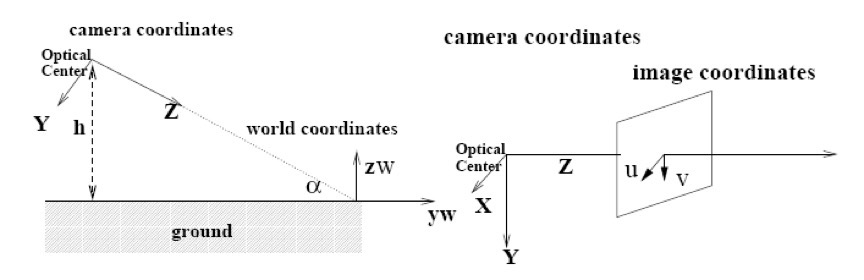
\includegraphics[width=0.7\linewidth]{coord.jpg}
    \caption{Coordinate System}
    \end{figure}
    \begin{solution}
        First of all, find the rotation matrix $R$ that maps points in world coordinate to the same points in camera coordinate. Since the rotation is about $x$ axis, it can be described by the matrix ($\theta$ is defined using right-hand rule):
        
        \begin{equation}
            \begin{split}
            R _ { x } ( \theta )
            & = \left[ \begin{array} { c c c } { 1 } & { 0 } & { 0 } \\ { 0 } & { \cos \theta } & { - \sin \theta } \\ { 0 } & { \sin \theta } & { \cos \theta } \end{array} \right] \\
            & = \left[ \begin{array} { c c c } { 1 } & { 0 } & { 0 } \\ { 0 } & { - \sin \alpha } & { - \cos \alpha } \\ { 0 } & { \cos \alpha } & { - \sin \alpha } \end{array} \right], \ \theta = \frac{\pi}{2} + \alpha 
        \end{split}
        \end{equation}
        
        Next, the translation vector is defined by the world origin expressed in the camera frame:
        \[ t = \left( \begin{array} {c} {0} \\ {0} \\ {\frac{h}{\sin \alpha}} \\ \end{array} \right) \]
        
        Composite the Euclidean transformation described in Eq. (2) and the perspective projection described in Eq. (1):
        \[ 
        \begin{split}
            M 
            &= \left[ \begin{array} { l l l l } { f } & { 0 } & { 0 } & { 0 } \\ { 0 } & { f } & { 0 } & { 0 } \\ { 0 } & { 0 } & { 1 } & { 0 } \end{array} \right] \left[ \begin{array} { c c c c } { 1 } & { 0 } & { 0 } & { 0 } \\ { 0 } & { - \sin \alpha } & { - \cos \alpha } & { 0 } \\ { 0 } & { \cos \alpha } & { - \sin \alpha } & { \frac{h}{\sin \alpha} } \\ { 0 } & { 0 } & { 0 } & { 1 } \end{array} \right] \\
            &= \left[ \begin{array} { l l l l } { f } & { 0 } & { 0 } & { 0 } \\ { 0 } & { -f\sin\alpha } & { -f\cos\alpha } & { 0 } \\ { 0 } & { \cos \alpha } & { -\sin \alpha } & { \frac{h}{\sin \alpha} } \end{array} \right] \\
        \end{split}
        \]
    With this, 
    \end{solution}
    
    \subpart
    * Find the $3 \times 3$ matrix for the linear transformation that maps points on the world plane $Z_w = d$ to the image plane $(u, v, w)$.
    \begin{solution}
        Borrowing the result from part (ii):
        \[
        \begin{split}
        \left( \begin{array} { c } { u } \\ { v } \\ { w } \end{array} \right) 
        &= M \left( \begin{array} { c } { X _ { w } } \\ { Y _ { w } } \\ { Z _ { w } } \\ { 1 } \end{array} \right) \\
        &= \left[ \begin{array} { l l l l } { f } & { 0 } & { 0 } & { 0 } \\ { 0 } & { -f\sin\alpha } & { -f\cos\alpha } & { 0 } \\ { 0 } & { \cos \alpha } & { -\sin \alpha } & { \frac{h}{\sin \alpha} } \end{array} \right] \left( \begin{array} { c } { X _ { w } } \\ { Y _ { w } } \\ { d } \\ { 1 } \end{array} \right) \\
        &= \left( \begin{array} { c } { f X _ { w } } \\ { - f Y _ { w } \sin \alpha - f d \cos \alpha } \\ { Y _ { w } \cos \alpha - d \sin \alpha + \frac{h}{\sin \alpha} } \end{array} \right) \\
        \end{split}
        \]
    We need to convert this into a $M ^ {'} _ {3 \times 3} \left( \begin{array} {c} X _ {w} \\ Y _ {w} \\ 1 \\ \end{array} \right)$ form:
    \[  \left( \begin{array} { c } { u } \\ { v } \\ { w }            \end{array} \right) = \begin{bmatrix}
        f & 0 & 0 \\
        0 & -f\sin \alpha & -fd \cos \alpha \\
        0 & \cos \alpha & \frac{h}{\sin \alpha} - d \sin \alpha \\
        \end{bmatrix}
        \left( \begin{array} {c} {X _ {w}} \\ {Y _ {w}} \\ {1} \\ \end{array} \right) \\
    \]

    \end{solution}
\end{subparts}


\end{parts}
\end{questions}
\clearpage

\section{Singular Value Decomposition for Image Compression and PCA}
\begin{questions}
\question{
  Many thousands of outdoor cameras are currently connected to the Internet. They can be used to measure plant growth (e.g. in response to recent warming trends), survey animal populations (e.g. in national parks), monitor surf conditions, and security, etc.
  In this question, you are provided with a 150-frame time-lapse video of a city scene taken between 6.30 - 7.30pm. Each frame is of the dimension 161x261 pixels. Watch the video, and you can see that clouds are moving, and planes take off and land from a nearby airport.
}
\begin{parts}

\part
Using Matlab, load the first image in the video sequence provided with this question and convert it to an appropriate data type (\mcode{I=im2double(imread(‘image001.png’));}).

\part
Do a singular value decomposition using the command ‘svd’: \mcode{[U S V]=svd(I);}
This will give you the singular values and the singular vectors. The singular values in S have been sorted in descending order. Plot the singular value spectrum using the command: \mcode{plot(diag(S),'b.')}. \textbf{Submit this plot. What do you notice in this plot?}

    \begin{figure}[!h]
    \centering
    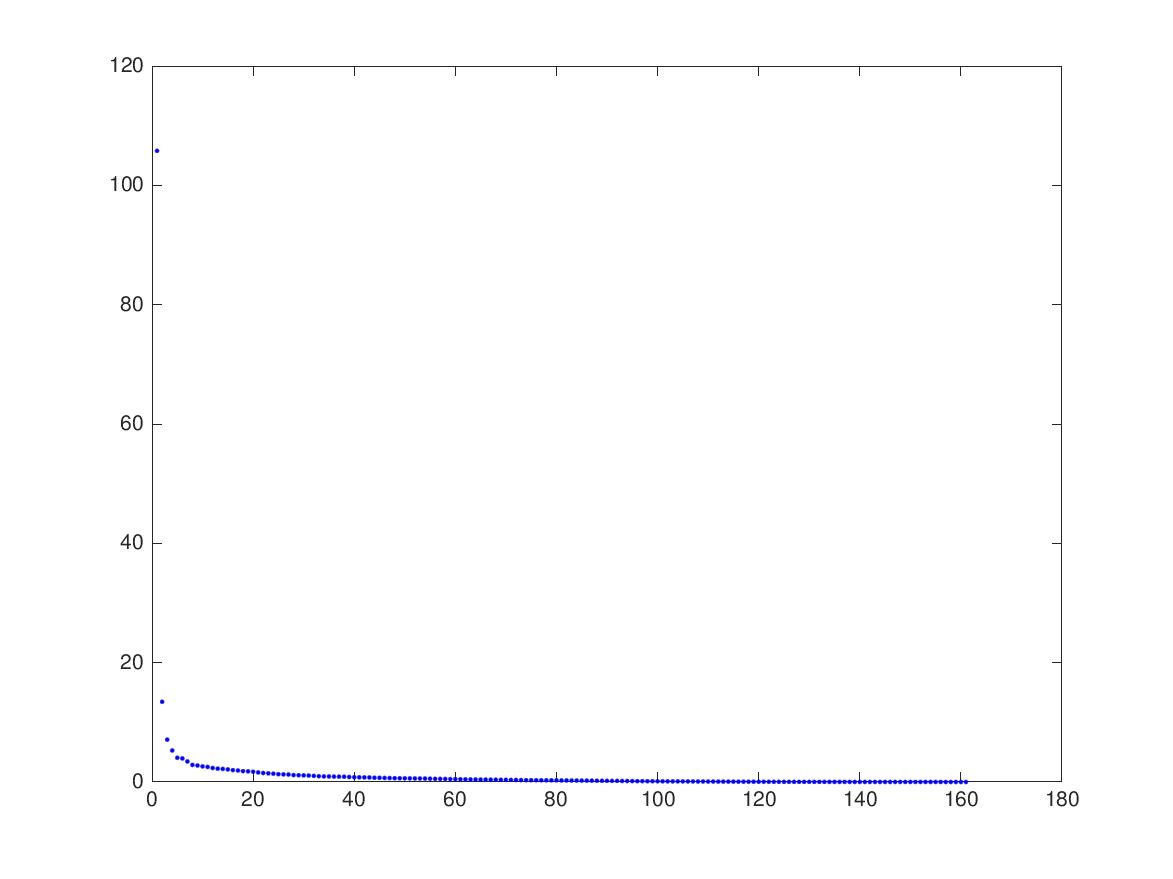
\includegraphics[width=0.7\linewidth]{SingularValues.jpg}
    \caption{Singular values}
    \end{figure}
    
\begin{solution}
    All the singular values are plotted in Fig. 2.
    As shown, the first singular value is very large ($>100$), while the following singular values are approximately between $[5, 20]$. When the index gets even larger, the singular values approaches zero (become very small).
    The condition number, which is 
    \begin{equation}
        cond(I)=\frac{\sigma_{max}}{\sigma_{min}}
    \end{equation}
    gets very large as a result. This suggests that it is ill-conditioned.

\end{solution}

\part
Let K=20, Extract the first K singular values and their corresponding vectors in U and V:

\begin{lstlisting}
K=20;
Sk=S(1:K,1:K);
Uk=U(:,1:K);
Vk=V(:,1:K);
\end{lstlisting}

Uk, Vk, Sk contain the compressed version of the image. To see this, form the compressed image:

\begin{lstlisting}
Imk=Uk*Sk*Vk';
imshow(Imk)
\end{lstlisting}

\textbf{Print out a copy of this compressed image and submit it.}
\begin{solution}
    The compressed image using the first 20 singular values is shown in Fig. 3 below.
\end{solution}

    \begin{figure}[!h]
    \centering
    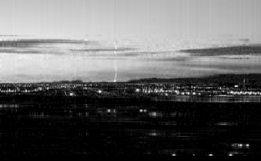
\includegraphics[width=0.7\linewidth]{k20_compressed001.png}
    \caption{Compressed image (K=20)}
    \end{figure}

\part
Repeat question (c) for K=40,60,80. \textbf{Submit the compressed images for the different values of K. Compare the 4 compressed images. Briefly describe what you notice.}
\begin{solution}
    The resultant images are shown in Fig. 4 - Fig. 6.
    As we take more singular values into computation (larger K), the quality of the compressed image improves. 
    \begin{equation}
        \Tilde{I} = s _ { 1 } u _ { 1 } v _ { 1 } ^ { T } + s _ { 2 } u _ { 2 } v _ { 2 } ^ { T } + \cdots + s _ { K } u _ { K } v _ { K } ^ { T }
    \end{equation}
    As shown in the equation above, larger K will give better approximation.

\end{solution}
    \begin{figure}[H]
    \centering
    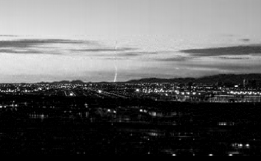
\includegraphics[width=0.6\linewidth]{k40_compressed001.png}
    \caption{Compressed image (K=40)}
    \end{figure}
    
    \begin{figure}[H]
    \centering
    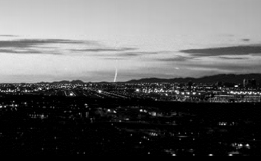
\includegraphics[width=0.6\linewidth]{k60_compressed001.png}
    \caption{Compressed image (K=60)}
    \end{figure}
    
    \begin{figure}[H]
    \centering
    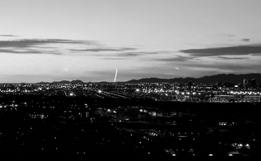
\includegraphics[width=0.6\linewidth]{k80_compressed001.png}
    \caption{Compressed image (K=80)}
    \end{figure}
\part
Thus, in image transmission, instead of transmitting the original image you can transmit $Uk, Vk, Sk$, which should be much less data than the original. \textbf{Is it worth transmitting when K=100} (i.e. do you save any bits in transmission when K=100)? Explain your answer.

\begin{solution}
    The total storage of the compressed image $I_{K}$ is expressed by:
    \begin{equation}
        S = K(m+n+1)
    \end{equation}
    For this question, $m=161, n=261$, so if we take $K=100$, the total storage we need for the transmission is $100 \times (161+261+1) = 42300$. This is even larger than the storage for just transmitting original image ($161 \times 261=42021$). Thus, transmitting compressed image with K=100 is \textbf{NOT} worth.
\end{solution}

\part
** Find an expression that bounds the per-pixel error (the difference between the original image and the compressed image for a particular pixel $(i, j)$) in terms of K, the singular values and the elements in U and V with the largest absolute magnitude $(u_{max}, v_{max}$ respectively).

\begin{solution}
    The completely re-constructed image (suppose $N$ non-zero singular values) and the compressed image using first K singular values are expressed by:
    \begin{equation}
        \begin{split}
            I 
            &= s _ { 1 } u _ { 1 } v _ { 1 } ^ { T } + s _ { 2 } u _ { 2 } v _ { 2 } ^ { T } + \cdots + s _ { K } u _ { K } v _ { K } ^ { T } + \cdots + s _ { n } u _ { n } v _ { n } ^ { T } \\
        \Tilde{I} 
        &= s _ { 1 } u _ { 1 } v _ { 1 } ^ { T } + s _ { 2 } u _ { 2 } v _ { 2 } ^ { T } + \cdots + s _ { K } u _ { K } v _ { K } ^ { T }
        \end{split}
    \end{equation}
    So the error term is their difference:
    \begin{equation}
        \varepsilon = |\sum_{n=K+1}^{N} s _ { n } u _ { n } v _ { n } ^ { T } |
    \end{equation}
    For a single pixel ($I_{i,j}$), the error is:
    \begin{equation}
        \begin{split}
        \epsilon 
        &= | \sum_{n=K+1}^{N} s _ { n } u _ { i, n } (v ^ { T })_{n, j} |\\
        &\leqslant \sum_{n=K+1}^{N} |s _ { n } u _ { i, n } (v ^ { T })_{n, j}|\\
        &\leqslant \sum_{n=K+1}^{N} s _ { n } |u _ { i, n }| |(v ^ { T })_{n, j}|\\
        &\leqslant \sum_{n=K+1}^{N} s _ { n } u _ { max } v _{max}\\
    \end{split}
    \end{equation}
    
\end{solution}

\part
** SVD is intimately related to PCA (Principal components analysis). Some of you might have learned about PCA in the EE3731C course, but it is not a pre-requisite for this question. Basically, finding the principal components of a matrix $X$ amounts to finding an orthonormal basis that spans the column space of $X$ (these are the column vectors $u_i$ in the matrix $U$). Here we create the data matrix $X$ by first vectorizing each of the 150 images into a column vector (by scanning in either row-major order or column- major order), and then stacking these vectors together into a matrix of size $42021\times150$. In effect, we have captured the entire video sequence into the 2D matrix $X$. \\\\
Before we proceed further, mean subtraction (a.k.a. "mean centering") to center the data at the origin is necessary for performing PCA. That is, the images are mean centered by subtracting the mean image vector from each image vector. This is to ensure that the first principal component $u_{1}$ really describes the direction of maximum variance. Again, if you do not have background in PCA, it is okay; just take it as a preprocessing step (or you can do some independent learning). \\\\
Apply SVD to the resultant mean-centered matrix. Take only the first $10$ principal components and reconstruct the image sequence. [NB: you can use the Matlab \mcode{reshape} command to convert a matrix to a vector and vice versa]. Observe the dynamics in the reconstructed video, comment on what you find, and explain why. Remember to add back this mean image vector when you are displaying your reconstructed results. \\\\
\text{[Non-mandatory]}: You can also explore other possibilities, like investigating what each principal component means, and their implications for processing and editing of outdoor webcam imagery.

\begin{solution}
    In principal component analysis we find the directions in the data with the most variation, i.e. the eigenvectors corresponding to the largest eigenvalues of the covariance matrix, and project the data onto these directions \cite{svd04}.
    
    Let's denote the elements in the data matrix $X$ as $X _ { j , \alpha } = x _ { j } ^ { \alpha }$. The mean vector is:
    \begin{equation}
        \langle \mathbf { x } \rangle \equiv \frac { 1 } { m } \sum _ { \alpha = 1 } ^ { m } \mathbf { x } ^ { \alpha }
    \end{equation}
    and the coariance matrix is:
    \begin{equation}
            C \equiv \frac { 1 } { m } \  X X  ^ { T },
    \end{equation}
    where we have removed the mean of the data: $X _ { j , \alpha } : = X _ { j , \alpha } - \left\langle x _ { j } \right\rangle$.
    
    Apply the SVD to $X$ and substitute $X$ in Eq. (11):
    \begin{equation}
        \begin{split}
            C &= \frac{1}{m} (U \Sigma V ^{T}) (U \Sigma V ^{T}) ^ {T}\\
            &= \frac{1}{m} U \Sigma V ^ {T} V \Sigma ^ {T} U ^ {T}\\
            &= \frac{1}{m} U \Sigma ^ {2} U ^ {T}
        \end{split}
    \end{equation}
    
    Clearly, the result in Eq. (12) demonstrates the Eigendecomposition of the real-valued symmetric matrix $mC$. Hence, the columns of $U$ are the eigenvectors of matrix $mC$ and the diagonal elements of $\Sigma ^ {2}$ are the eigenvalues. Therefore, the matrix $U$ after SVD of $X$ actually contains what we want for PCA. 
    
    Furthermore, if we denote the matrix of eigenvectors \textbf{sorted} according to eigenvalue by $\Tilde{U}$ , we can then use PCA to transform the data to be ${ Y } = \tilde {  U  } ^ { T }  { X }$. The eigenvectors are called the principal components. By selecting only the first $d$ rows of $Y$, we have projected the data from $n$ down to $d$ dimensions. \\\\
    In Matlab, to load all the images and construct the data matrix $X$, and do the mean subtraction:
    \begin{lstlisting}
X = [];
Files=dir('*.png');
for k=1:length(Files)
   FileNames=Files(k).name;
   I = im2double(imread(FileNames));
   I = I(:);
   X = [X I];
end
mean_X = mean(X, 2);
de_mean_X = X - mean_X;
    \end{lstlisting}
    Then, to calculate the SVD of matrix $X$ and transform the data into the first $10$ principle components' space:
    \begin{lstlisting}
[U S V] = svd(de_mean_X,0); % to produce "economy size"
X_PCAed = U(:,1:10) * S(1:10, :) * V';
X_reconstructed = X_PCAed + meanX;
for i=1:150
    Mat = X_reconstructed(:,i);
    Name = strcat('img_', int2str(i), '.png');
    imwrite(reshape(Mat, [161, 261]) ,Name,'png');
end
    \end{lstlisting}
    \textbf{Findings}\\
    By viewing the reconstructed video, I found that the only the light generated by planes sliding on the ground remains, while the light during the landing and taking off processes are nearly ``removed out". Besides, the light also gets blurry after PCA operation. This is because the operation only takes the first ten largest singular values out as valid information, and forms the orthogonal basis using these corresponding eigen-vectors. Every single image (column) is reconstructed using the principle components of all the images thus only the ``common" information remains; and between the frames (row) they are also ``smoothed out" thus things get blurry.
    
\end{solution}
\end{parts}
\end{questions}
\clearpage

\section{Projection Model, Homogeneous coordinates}
\begin{questions}
\question
\begin{parts}
\part
An affine camera is a simplification of the full perspective camera but is more complicated than the scaled orthographic model. It has a projection relationship given by the following equations: $\left(\begin{array}{c} x \\ y \\ \end{array}\right) = A\left(\begin{array}{c}X\\Y\\Z\\ \end{array}\right) + \mathbf{b}$, where $A$ is a $2 \times 3$ matrix, and $\mathbf{b}$ is a vector in $\mathcal{R}^{2}$. If the world point $(X, Y, Z)^{T}$ and the image point $(x, y)^{T}$ are represented by homogeneous vectors, write down the matrix representing the linear mapping between their homogeneous coordinates. \\\\
* Show that the point at infinity in space $(X, Y, Z, 0)^{T}$ is mapped to point of infinity in the image plane. What does this result imply about the projection of parallel lines in space onto the image plane?

\begin{solution}
    Similar to Eq. (2), in the homogeneous coordinate, affine transformation is described by:
    \begin{equation}
    \begin{split}
        \left(\begin{array}{c} x \\ y \\ 1 \\ \end{array}\right) 
        &= \begin{bmatrix}
        A & \mathbf{b} \\
        \mathbf{0} ^ {T} & 1
        \end{bmatrix}
        \left(\begin{array}{c}X\\Y\\Z\\1\\ \end{array}\right) \\
        &= H _ {A} \left(\begin{array}{c}X\\Y\\Z\\1\\ \end{array}\right) \\
    \end{split}
    \end{equation}
    
    To show the required statement, just apply the affine transformation $H_{A}$ to $(X, Y, Z, 0)^{T}$, we obtain $(x', y', 0)$ in the image plane. The result indicates that this point is at infinity in the image plane.
    
    We know that the intersection of two parallel lines is at infinity in the 3-D space. So this result implies that after affine transformation, the intersection point is still at the infinity in the image plane. This is because affine transformation is parallelity-invariant.
    

\end{solution}

\part
Given an image of a scene containing a cube as shown in the
following. 
    \begin{figure}[H]
    \centering
    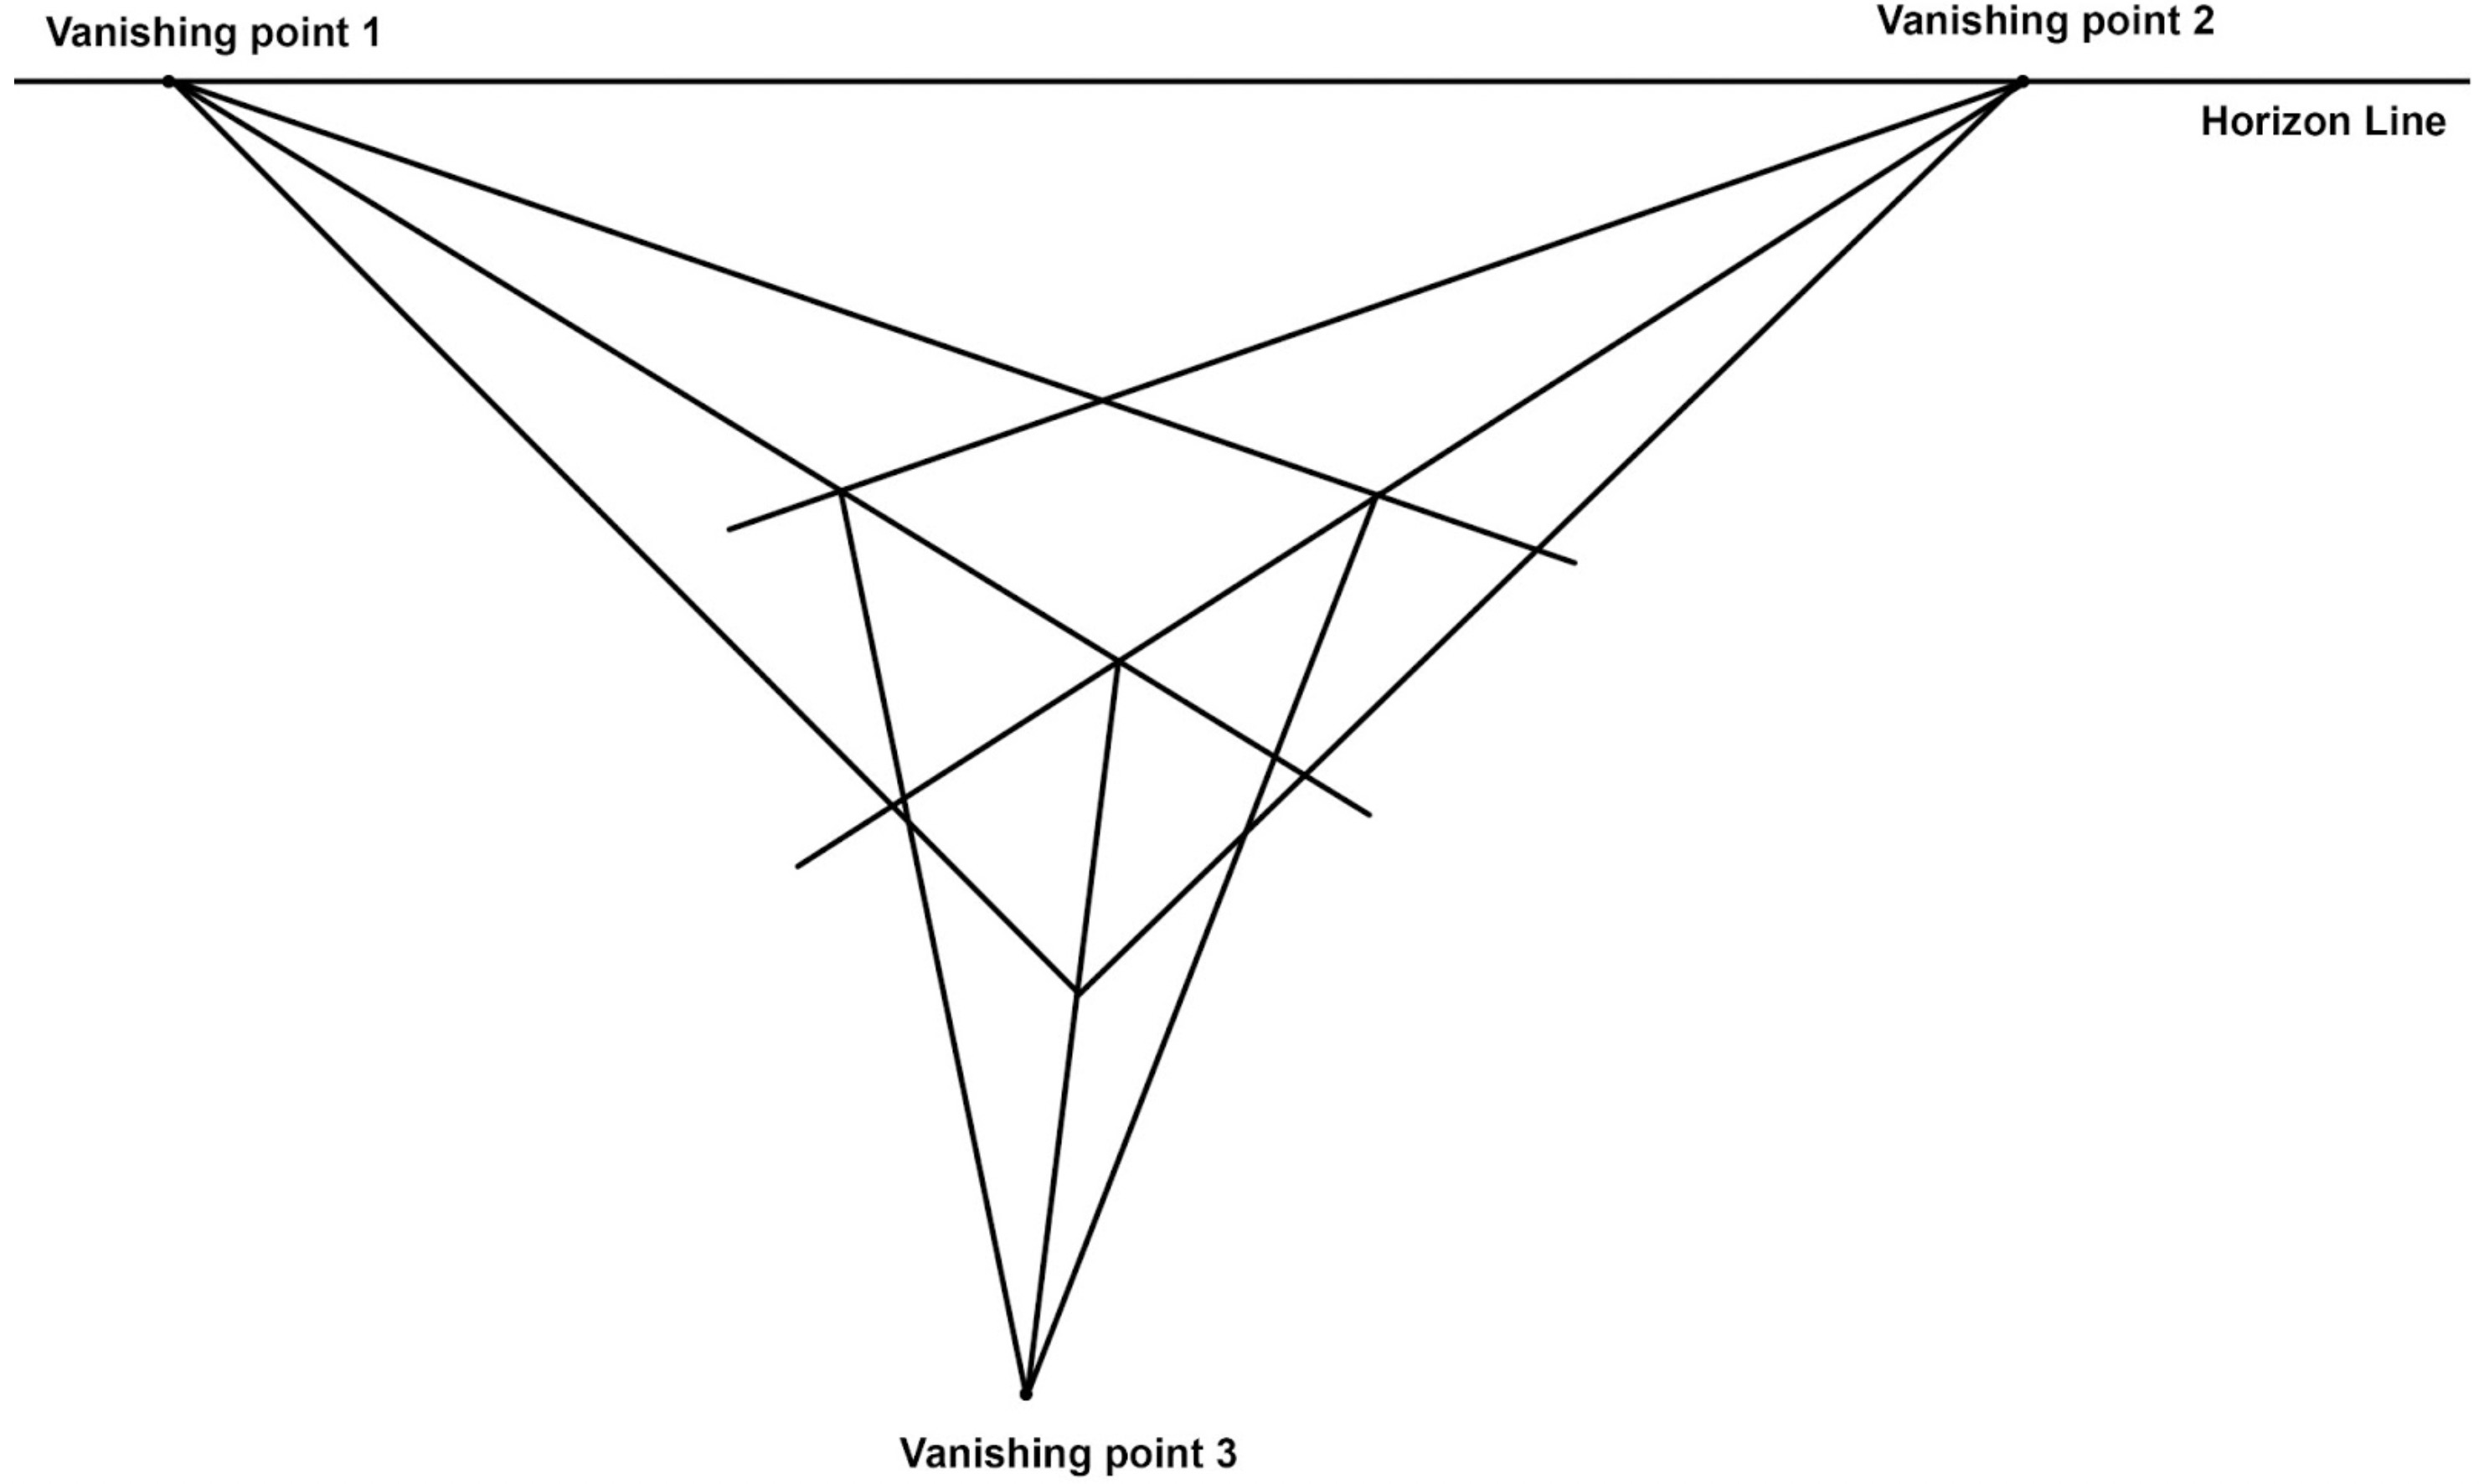
\includegraphics[width=0.5\linewidth]{cube.jpeg}
    \caption{Cube}
    \end{figure}
Each vanishing point is the point on the image corresponding to a point in 3D space at infinity of the form $(\mathbf{d}, 0) ^ {T}$, where $\mathbf{d}$ is a Euclidean vector with 3 coordinates expressing the direction of a cube edge. 
\begin{subparts}
    \subpart
    ** Show that the coordinates of a vanishing point $\mathbf{v}$ can be expressed as $\mathbf{v} = K R \mathbf{d}$, where $K$ is the intrinsic calibration matrix and $R$ is the rotation matrix between the camera and world coordinate system. Hence express an edge direction $\mathbf{d}$ as a function of K, R and $\mathbf{v}$. (Hint: Start from the $3\times4$ projection matrix equation in Ch 1)
    
    \begin{solution}
        Let $\mathbf{d}=(a, b, c) ^ {T}$, and apply the projection matrix to point at infinity in 3D space $x _ {\infty} = (a, b, c, 0) ^ {T}$:
        \begin{equation}
                    \begin{split}
            \mathbf{v} &= M x _ {\infty} = K \left[R \quad T\right] \left( \begin{array}{c}
                 a  \\
                 b  \\
                 c  \\
                 0
            \end{array} \right) \\
            &= K R \left( \begin{array}{c}
                 a  \\
                 b  \\
                 c  
            \end{array} \right) \\
            &= K R \mathbf{d}
        \end{split}
        \end{equation}
        Hence, the direction vector is:
        \begin{equation}
            \mathbf { d } = \frac { (KR) ^ { - 1 }   \mathbf{v}  } { \left\| (KR) ^ { - 1 }  \mathbf{v}  \right\| }
        \end{equation}
        
        
    \end{solution}
    
    \subpart
    ** The 3 directions of the cube edges are mutually perpendicular; therefore the dot product between any two directions is zero. Show that this condition leads to an equation in terms of the vanishing points and the unknown calibration matrix $K$. Note that such an equation can be written for each pair of the 3 vanishing points.
    
    \begin{solution}
        First, the angle between any two directions in the 3D space is given by the cosine rule:
        \begin{equation}
            \begin{aligned} \cos \theta & = \frac { \mathbf{d} _ { 1 } \cdot \mathbf{d} _ { 2 } } { \left\| \mathbf{d} _ { 1 } \right\| \left\| \mathbf{d} _ { 2 } \right\| } \\ & = \frac { v _ { 1 } ^ { T } \omega v _ { 2 } } { \sqrt { v _ { 1 } ^ { T } \omega v _ { 1 } } \sqrt { v _ { 2 } ^ { T } \omega v _ { 2 } } } \end{aligned}
        \end{equation}
        where $\omega = \left( (KR) (KR) ^ { T } \right) ^ { - 1 } = \left( K K ^ { T } \right) ^ { - 1 }$.
        
        As given, all the edges are mutually perpendicular, therefore $\cos \theta = 0$, and the equations given by these three vanishing points are:
        \begin{equation}
            v  _ { 1 } ^ { T  } \omega  v  _  2  = v  _ { 1 } ^ { T  } \omega  v  _  {3} = v  _ { 3 } ^ { T  } \omega  v  _  {3} =0
        \end{equation}
    \end{solution}
    
    \subpart
    *** Note that the derived equation above can be used to solve for K, but you are not required to explicitly propose a scheme for solving this equation. However, doing so will earn you bonus point.
    
    \begin{solution}
        In this setup, we have three constraints, but the unknown $K$ has five degrees of freedom. Hence, we could make assumption that the camera has zero-skew and square pixels to add two more constraints on it.
        
        Our original intrinsic matrix is given by:
        \begin{equation}
            K = \left[ \begin{array} { c c c } { \frac { - 1 } { s _ { x } } } & { k } & {  { o } _ { x } } \\ { 0 } & { \frac { - 1 } { S _ { y } } } & {  { o } _ { y } } \\ { 0 } & { 0 } & { 1 } \end{array} \right]
        \end{equation}
        
        By the additional constraints, it becomes:
        \[
            K = \left[ \begin{array} { c c c } { \alpha } & { 0 } & {  { o } _ { x } } \\ { 0 } & { \alpha } & {  { o } _ { y } } \\ { 0 } & { 0 } & { 1 } \end{array} \right]
        \]
        Therefore, with three equations, to solve three unknowns becomes possible. And by doing this we calibrate the camera with a single image!
    \end{solution}
\end{subparts}

\part
The projection of a scene point in world coordinates to pixel coordinates in an image can be represented using a camera projection matrix $P$ as follows:
\[
\left( \begin{array} { c } { s _ u } \\ { s _ v } \\ { s } \end{array} \right) = \left[ \begin{array} { l l l l } { p _ { 11 } } & { p _ { 12 } } & { p _ { 13 } } & { p _ { 14 } } \\ { p _ { 21 } } & { p _ { 22 } } & { p _ { 23 } } & { p _ { 24 } } \\ { p _ { 31 } } & { p _ { 32 } } & { p _ { 33 } } & { p _ { 34 } } \end{array} \right] \left( \begin{array} { c } { X _ { w } } \\ { Y _ { w } } \\ { Z _ { w } } \\ { 1 } \end{array} \right)
\]
\begin{subparts}
    \subpart
    * Given a set of lines in a scene that are all parallel to the world $X$-axis, what is the vanishing point, $(u, v)$, of these lines in the image? Can you conclude whether an infinite line in 3D space always yield an infinite line in the 2D image plane?
    
    \begin{solution}
        Let a point at infinity in 3D space $x_{\infty} = (1, 0, 0, 0) ^ {T}$.
        Apply the projection matrix $P$, we obtain the corresponding image point:
        \[
        \left( \begin{array} { c } { s _ u } \\ { s _ v } \\ { s } \end{array} \right) = \left( \begin{array} { c } { p_{11} } \\ { p_{21} } \\ { p_{31}} \end{array} \right)
        \]
        As we can observe, an infinite line in 3D space dons \textbf{not} necessarily yield an infinite line in 2D image plane, since the $s$ component may be non-zero. For example, if the projection is an affine transformation, the image line will be at infinity; however, is the projection is an projective transformation, the image line will not be at infinity.
    \end{solution}
    
    \subpart
    What is the significance of the image point (represented as a homogeneous 3-vector) given by the last column $(p _ {14}, p_ {24}, p_ {34})$ of $P$? That is,which world point gives rise to  $(p _ {14}, p_ {24}, p_ {34})$ ?
    
    \begin{solution}
        If the world point is $(0,0,0,1) ^ {T}$, the corresponding image point will be $(p _ {14}, p_ {24}, p_ {34})$. Actually is the image point of the plane at infinity $\Pi _ {\infty} = (0,0,0,1) ^ {T}$, and it's also referred as \textbf{horizon line}. 
    \end{solution}
    
    \subpart
    ** Consider the 1-dimensional right null-space of $P$, i.e., the 4-vector $\mathbf{C}$ such that $P \mathbf{C}=0$. In this case, the image point of $\mathbf{C}$ is $(0, 0, 0) ^ {T}$ which is not defined. What is the point $\mathbf{C}$ which possesses this property? Explain.
    
    \begin{solution}
        Point $\mathbf{C}$ should be the camera center.
        \begin{proof}
            Let $\mathbf{A}$ be an arbitrary point in the 3D space. A line can be formed by connecting point $\mathbf{A}$ and point $\mathbf{C}$. Points on this line can be described by:
            \begin{equation}
                \mathbf { X } ( \lambda ) = \lambda \mathbf { A } + ( 1 - \lambda ) \mathbf { C } , - \infty < \lambda < \infty
            \end{equation}
            Under the projection $ \mathbf { x } = P \mathbf { X }$, the image point on this line can be described by:
            \begin{equation}
                \mathbf { x } = P \mathbf { X } ( \lambda ) = \lambda \mathrm { P } \mathbf { A } + ( 1 - \lambda ) \underbrace { P \mathbf { C } } _ { = 0 } = \lambda \mathrm { P } \mathbf { A } , - \infty < \lambda < \infty
            \end{equation}
            Eq. (20) shows that all the points on this 3D line are mapped to the same point. Thus this line must go through the camera center. Additionally, since point $\mathbf{A}$ is arbitrary, to make sure the line goes through the camera center, point $\mathbf{C}$ must be the camera center.
        \end{proof}
    \end{solution}
\end{subparts} 

    \part
    The equation of a conics in inhomogeneous coordinates is given by $a x ^ { 2 } + b x y + c y ^ { 2 } + d x + e y + f  = 0$. 
    \begin{subparts}
        \subpart
        Homogenize this equation by the replacement $ x \rightarrow \frac{x_{1}}{x_{3}} $, $ y \rightarrow \frac{x_{2}}{x_{3}} $, and write down the homogeneous form. Finally, express this homogeneous form in the matrix form $\mathbf { x } ^ {  T  }  \mathrm { C }  \mathbf { x } = 0$, where $\mathrm { C }$ is symmetric. Write down the elements of the symmetric matrix $\mathrm { C }$.
        
        \begin{solution}
            In homogeneous coordinate, the conics equation becomes:
            \begin{equation}
                a x _ { 1 } ^ { 2 } + b x _ { 1 } x _ { 2 } + c x _ { 2 } ^ { 2 } + d x _ { 1 } x _ { 3 } + e x _ { 2 } x _ { 3 } + f x _ { 3 } ^ { 2 } = 0
            \end{equation}
            This can be written in matrix form:
            \begin{equation}
                \left( \begin{array} {c c c} {x _ {1}} & {x _ {2}} & {x _ {3}}  \end{array} \right) \left[ \begin{array} { c c c } { a } & { b / 2 } & { d / 2 } \\ { b / 2 } & { c } & { e / 2 } \\ { d / 2 } & { e / 2 } & { f } \end{array} \right] \left( \begin{array} {c} x _ {1} \\ x _ {2} \\ x _ {3} \end{array} \right) = 0
            \end{equation}
            So the symmetric conics matrix $\mathrm { C } = \left[ \begin{array} { c c c } { a } & { b / 2 } & { d / 2 } \\ { b / 2 } & { c } & { e / 2 } \\ { d / 2 } & { e / 2 } & { f } \end{array} \right]$.
        \end{solution}
        
        \subpart
        ** If $\mathrm { C }$ has the special form $\mathrm { C } = \mathbf{l} \mathbf{m} ^ {T} + \mathbf{m} \mathbf{l} ^ {T}$ , clearly $\mathrm { C }$ is symmetric and therefore represents a conic. Show that the vector $\mathbf{x} = \mathbf{l} \times \mathbf{m}$ is the null vector of $\mathrm { C }$. Since a null vector exists, $\mathrm { C }$ is a degenerate conic. Show in this degenerate case, $\mathrm { C }$ contains two lines $\mathbf{l}$ and $\mathbf{m}$, that is, show that the points on the lines $\mathbf{l}$ and $\mathbf{m}$ satisfy $\mathbf { x } ^ { T }   \mathrm{C}  \mathbf { x } = 0$.
        
        \begin{solution}
            We know that in homogeneous coordinate, $\mathbf{x} = \mathbf{l} \times \mathbf{m}$ means that $x$ is the intersection of lines $\mathbf{m}$ and $\mathbf{l}$. Thus we have:
            \begin{equation}
                \mathbf{m} ^ {T} \mathbf{x} = 0, \quad \mathbf{l} ^ {T} \mathbf{x} = 0
            \end{equation}
            Therefore, to show that $\mathbf{x}$ is the null vector of $\mathrm { C }$:
            \begin{equation}
                    \mathrm { C } \mathbf{x} = \mathbf{l} \mathbf{m} ^ {T} \mathbf{x} + \mathbf{m} \mathbf{l} ^ {T} \mathbf{x} = \mathbf{0}
            \end{equation}
            
            Since conic $\mathrm{C}$ has a null vector, the matrix $\mathrm{C}$ is not of full rank, and it is a degenerate conic. To show line $\mathbf{l}$ is on this conic, let $\mathbf{p}$ be any arbitrary point on line $\mathbf{l}$, we have $\mathbf{l} ^ {T} \mathbf{p} = \mathbf { p } ^ { T } \mathbf { l }  = 0$. To evaluate $\mathbf{p} ^ {T} \mathrm{C} \mathbf{p}$:
            \begin{equation}
                \mathbf { p } ^ { T } \mathrm { C } \mathbf { p } = \left( \mathbf { p } ^ { T } \mathbf { l } \right) \left( \mathbf { m } ^ { T } \mathbf { p } \right) + \left( \mathbf { p } ^ { T } \mathbf { m } \right) \left( \mathbf { l } ^ { T } \mathbf { p } \right) = 0
            \end{equation}
            This shows $\mathbf{p}$ is on this conic. Since $\mathbf{p}$ is any arbitrary point on line $\mathbf{l}$, line $\mathbf{l}$ is on this conic.
            
            Using the similar steps for line $\mathbf{m}$ ($\mathbf{m} ^ {T} \mathbf{p} = \mathbf { p } ^ { T } \mathbf { m }  = 0$), we can get the same result as Eq. (25). 
            
            Thus, we can conclude that this degenerate conic contains two lines $\mathbf{l}$ and $\mathbf{m}$, and their intersection is the null vector for conic matrix $\mathrm{C}$.
        \end{solution}
    \end{subparts}
    
    \part
    Given a set of two-dimensional points $(x,y)$ as follows (not listed here, can be found in $conics.txt$), write a Matlab routine to find the conics best (in the least squares sense) represented by these points, in terms of the parameters $a, b, c, d, e,$ and $f$, as formulated in Question $3(d)$.
    
    \begin{solution}
        Any point $(x _ {i} , y _ {i})$ on the conic should satisfy the conic equation:
        \begin{equation}
            a x _ {i} ^ { 2 } + b x _ {i} y _ {i} + c y _ {i} ^ { 2 } + d x _ {i} + e y _ {i} + f  = 0
        \end{equation}
        This can be written as:
        \begin{equation}
            \left( \begin{array} { l l l l l l } { x _ { i } ^ { 2 } } & { x _ { i } y _ { i } } & { y _ { i } ^ { 2 } } & { x _ { i } } & { y _ { i } } & { 1 } \end{array} \right) \mathbf { c } = 0
        \end{equation}
        where $\mathbf { c } = ( a , b , c , d , e , f ) ^ { T }$ is the conic $\mathrm{C}$ as a 6-vector. This becomes a least square problem of the form $Ax=0$. The Matlab routine as below will find the ``best" conic:
        \begin{lstlisting}
load conics.txt
c = fit_conic(conics);
x = conics(:,1);
y = conics(:,2);
scatter(x,y)
hold on
fimplicit(@(x,y) c(1)*x^2 + c(2)*x*y + c(3)*y^2 + c(4)*x + c(5)*y + c(6))
xlabel('x')
ylabel('y')

function c = fit_conic(pts)
    x = pts(:,1);
    y = pts(:,2);
    A = [x.^2, x.*y, y.^2, x, y, ones(size(x))];
    [U, S, V] = svd(A);
    c = V(:,length(V)); % last column is the null vector
end
        \end{lstlisting}
        The result is verified in by plotting the figure below.
    \end{solution}
    \begin{figure}[H]
        \centering
        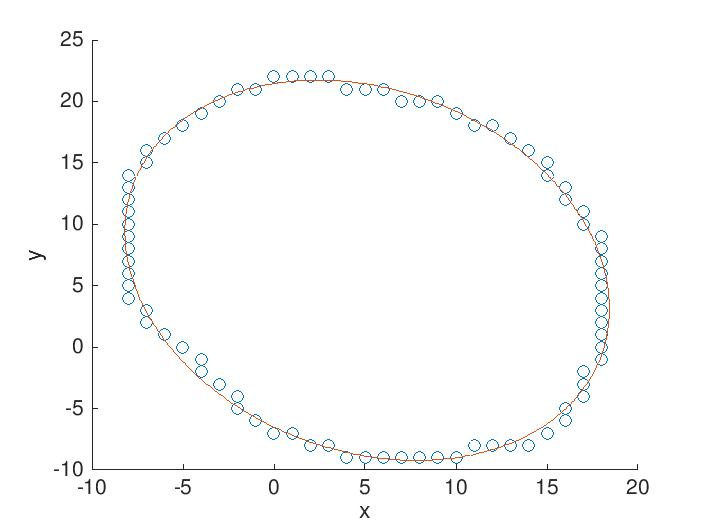
\includegraphics[width=0.6\linewidth]{conics_fitting.jpg}
    \end{figure}


\end{parts}
\end{questions}
\clearpage

\section{Estimate Fundamental Matrix F using 8-Point Algorithm}
\begin{questions}
\question
\textbf{Introduction}

The fundamental matrix F completely describes the epipolar geometry of a pair of images. 8-Point Algorithm is the simplest method for estimating the fundamental matrix. In this assignment, you will implement the 8-Point Algorithm to estimate the fundamental matrix given a pair of images. You would also need to implement the normalization so as to improve the stability (outlined in steps $4.2.2$ and $4.2.4$ below). Finally, we have also provided a package to help you reconstruct and visualize the depths (see point $6$ in $4.3$; this step is optional but will earn you bonus point). Please read this document completely before starting work. A list of reading materials you may need to solve this problem is given in Appendix I.

\question
\textbf{Tasks}

You are given 2 pairs of images (inria1.tif, inria2.tif, frc1.tif, frc2.tif) for this assignment. The steps for this assignment are:
\begin{enumerate}
    \item 
    Using one of the given pairs of images, establish $n (n \geq 8)$ point correspondences.
    
    \item
    Normalize the coordinates of the correspondences.
    
    \item
    Using the normalized coordinates of the correspondences, compute the fundamental matrix.
    
    \item
    Perform denormalization so as to find the fundamental matrix corresponding to the original data.
\end{enumerate}
Details of each step are given in the following sections. Some useful Matlab commands are given in Appendix II.

\begin{parts}
\part
\textbf[Establish Point Correspondences] \\
In this step, you need to establish point correspondences between the two images. Using Matlab, manually or automatically mark and record at least 8 pairs of corresponding points (preferably much more than 8 pairs for robustness!).

\begin{solution}
    After researching online, I used feature matching function provided in Matlab Computer Vision System toolbox based on \textbf{Harris Features} to \textbf{automatically} extract feature-matched points:
    
    \begin{lstlisting}
I1 = imread('frc1.jpg');
I2 = imread('frc2.jpg');

points1 = detectHarrisFeatures(I1, 'MinQuality', 0.001);
points2 = detectHarrisFeatures(I2, 'MinQuality', 0.001);

[features1,valid_points1] = extractFeatures(I1,points1);
[features2,valid_points2] = extractFeatures(I2,points2);

indexPairs = matchFeatures(features1,features2);

matchedPoints1 = valid_points1(indexPairs(:,1),:);
matchedPoints2 = valid_points2(indexPairs(:,2),:);


rand1 = randsample(32, 8);
grp1a = matchedPoints1(rand1);
grp1b = matchedPoints2(rand1);
grp1a = grp1a.Location;
grp1b = grp1b.Location;

rand1 = randsample(32, 8);
grp2a = matchedPoints1(rand1);
grp2b = matchedPoints2(rand1);
grp2a = grp2a.Location;
grp2b = grp2b.Location;

rand1 = randsample(32, 8);
grp3a = matchedPoints1(rand1);
grp3b = matchedPoints2(rand1);
grp3a = grp3a.Location;
grp3b = grp3b.Location;
    \end{lstlisting}
    Running the scripts above, I obtained three sets of points, each of which contains 8 point correspondences. As required by the question, I repeated the process of computing the fundamental matrix to check for the accuracy.
    
    The Figure $9 - 11$ below shows three different sets of matched points. These points are all corresponding \textbf{corners} on both images. They are chosen as the feature points to do the matching since they are less ambiguous compared to plain areas or edges.
    
    \begin{figure}[H]
        \centering
        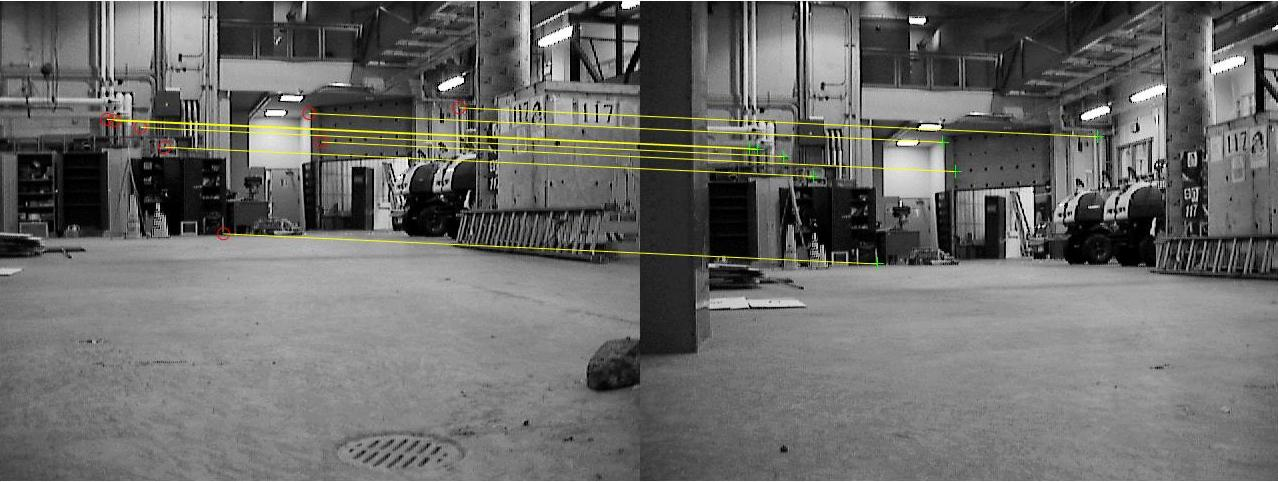
\includegraphics[width=0.75\textwidth]{grp1.jpg}
        \caption{$1 ^{st}$ set of point correspondences}
        \label{fig:mesh1}
    \end{figure}
    
    \begin{figure}[H]
        \centering
        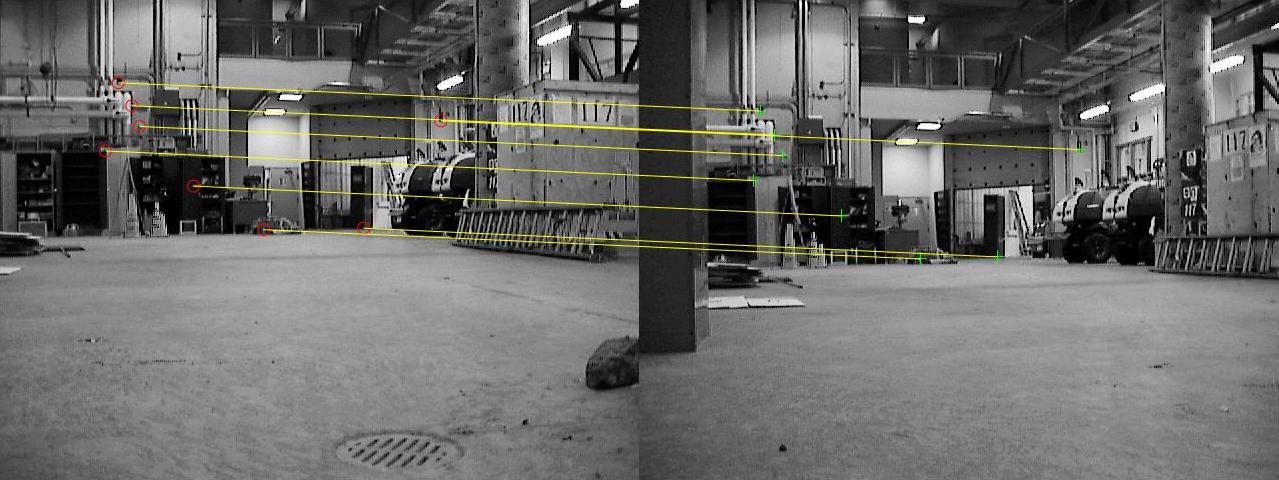
\includegraphics[width=0.75\linewidth]{grp2.jpg}
        \caption{$2 ^{nd}$ set of point correspondences}
    \end{figure}
    
    \begin{figure}[H]
        \centering
        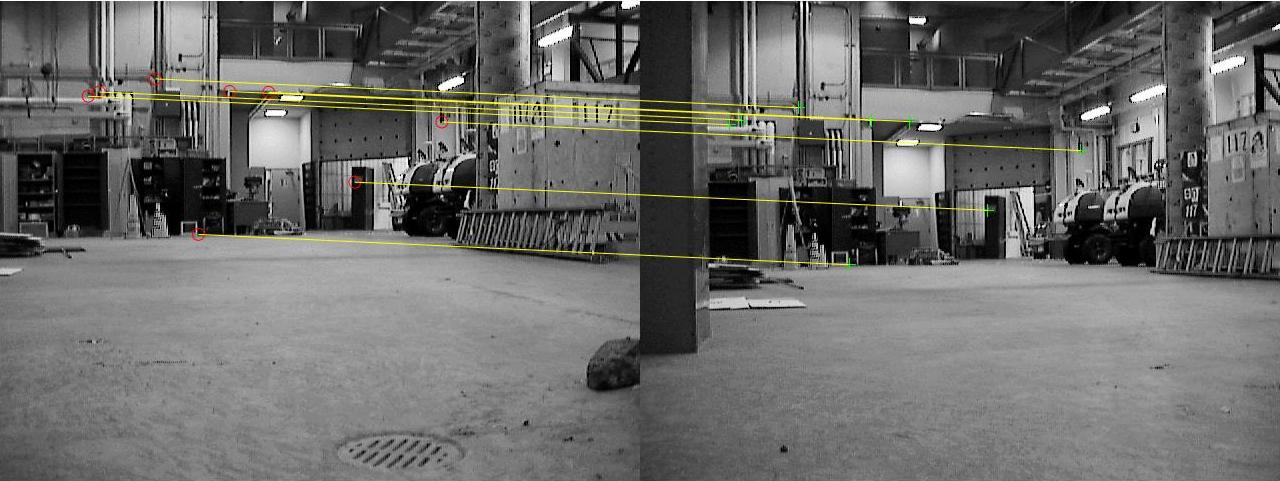
\includegraphics[width=0.75\linewidth]{grp3.jpg}
        \caption{$3 ^{rd}$ set of point correspondences}
    \end{figure}
    
\end{solution}

\part
\textbf[Normalization of the data] \\
In 8-point algorithm, the stability of the results can be greatly improved by a simple normalization (translation and scaling) of the coordinates of the correspondences (originally presented in [Hartley- 1997] and also in [Hartley and Zisserman-2000]). For this normalization, you should find a similarity transformation $T$ , consisting of a translation and scaling, that takes points $x_{i}$ to a new set of points $\hat{x} _ {i}$ ($\hat { x } _ { i } = T x _ { i }$ )such that the centroid of the points $\hat { x } _ { i }$ is the coordinates origin, and their average distance
(Root Mean Squares) from the origin is $2$ pixels . Similarly, find a similarity transformation $T'$ that takes points $x' _ {i}$ to points $xˆ_{i}$ ($\hat {  { x } } _ { i } ^ { \prime } = T ^ { \prime }  { x } _ { i }$).
Note: Homogeneous coordinates are used in this step.
\begin{solution}
    For one image, the centroid of all points is defined by:
    \begin{equation}
        (x_{c}, y_{c}) = (\frac{1}{N} \sum ^ {N} _ {i=1} x _ {i}, \frac{1}{N} \sum ^ {N} _ {i=1} y _ {i})
    \end{equation}
    Every point is translated such that the centroid of the points becomes the coordinate origin. The translation is determined by the centroid's coordinates:
    \begin{equation}
    \begin{split}
        t_{x} = - &x _{c}, \quad t_{y} = - y _{c} \\
        x _ {i} &:= x_{i} + t_{x} \\
        y _ {i} &:= y_{i} + t_{y} \\
    \end{split}
    \end{equation}
    
    After the translation, all the points are scaled such that their Root Mean Square distance from the origin is $\sqrt{2}$, which is equivalent to be scaled by $s$:
    \begin{equation}
        s = \sqrt{\frac{2}{\frac{1}{N} \sum ^ {N} _ {i=1} (x_{i} ^ {2} + y_{i}^{2})} }
    \end{equation}
    Hence, to write the transformation $\hat{x} _ {i} = s (x_{i} + t_{x})$ and $\hat{y} _ {i} = s (y_{i} + t_{y})$ in matrix form:
    \begin{equation}
        T _ {s} = 
        \begin{bmatrix}
        s & 0 & st_{x} \\
        0 & s & st_{y} \\
        0 & 0 & 1
        \end{bmatrix}
    \end{equation}
    The Matlab codes are listed in the next sectioon together with the codes for $F$ estimation.
   
\end{solution}

\part
\textbf[Computation of Fundamental Matrix] \\
The computation of the fundamental matrix is described in detail in your textbook or in Section 10.1 of [Hartley and Zisserman-2000]. In summary the steps are as follows:
\begin{subparts}
    \subpart
    Find the solution for $f$ \\
    From a set of n point correspondences, we obtain a set of linear equations of the form:
    \begin{equation}
        A f = \left[ \begin{array} { c c c c c c c c c} { x^ { \prime } _ { 1 } x _ { 1 } } & { x^ { \prime } _ { 1 } y _ { 1 } } & { x _ { 1 } ^ { \prime } } & { y _ { 1 } ^ { \prime } x _ { 1 } } & { y _ { 1 } ^ { \prime } y _ { 1 } } & { y _ { 1 } ^ { \prime } } & { x _ { 1 } } & { y _ { 1 } } & { 1 } \\ { \vdots } & { \vdots } & { \vdots } & { \vdots } & { \vdots } & {\vdots } & { \vdots }& { \vdots } & { \vdots } \\ { x^ { \prime } _ { n } x _ { n } } & { x^ { \prime } _ { n } y _ { n } } & { x _ { n } ^ { \prime } } & { y _ { n } ^ { \prime } x _ { n } } & { y _ { n } ^ { \prime } y _ { n } } & { y _ { n } ^ { \prime } } & { x _ { n } } & { y _ { n } } & { 1 } \end{array} \right] f = 0
    \end{equation}
    
    $A$ is an $n \times 9$ matrix ($n \geq 8$)and $f$ is the 9-vector made up of the entries of $F$ in row-major order. If $rank(A) \leq 8$, non-trivial solution for the system above exists, and if $rank (A) = 8$ , the solution is unique (up to scale). The solution for $f$ should be the last column of $V$ in the $svd(A) = U \Sigma V^{T}$ .
    
    \subpart
    Enforce singularity constraint\\
    Fundamental Matrix is singular, in fact of rank 2. The matrix $F$ found by the above method will not in general have rank 2 and steps should be taken to enforce this singularity constraint. One easy way to do this is: let $F=U \Sigma V^{T}$ be the SVD of $F$, where $\Sigma$ is a diagonal matrix $diag(r,s,t)$ satisfying $r \geq s \geq t$. Let
    $F^{\prime}=U diag(r,s,0) V^{T}$ . According to the so-called Frobenius norm, $F^{\prime}$ is the closest singular matrix to $F$. Thus replace $F$ by $F^{\prime}$. Note that you should use the normalized data.
    \begin{solution}
        The codes are listed as follows:
        \begin{lstlisting}
% construct A; assume normalized points are stored in n_pts1 and n_pts2
A = [n_pts2(:,1).*n_pts1(:,1) n_pts2(:,1).*n_pts1(:,2) n_pts2(:,1) n_pts2(:,2).*n_pts1(:,1) n_pts2(:,2).*n_pts1(:,2) n_pts2(:,2) n_pts1(:,1) n_pts1(:,2) ones(size(n_pts1(:,1)))];
% from svd(A), get F
[U, S, V] = svd(A);
F = V(:,length(V));
F = reshape(F, [3,3])';
% enforce F singularity
[U_f, S_f, V_f] = svd(F);
S_f(3,3) = 0;
F_prime = U_f * S_f * V_f';
        \end{lstlisting}
    \end{solution}
    
    \subpart
    Denormalization\\
    Till this step, you have obtained the fundamental matrix corresponding to the normalized data $\hat {  { x } } _ { i } \leftrightarrow \hat { { x } } ^ {\prime}_ { i }$. This needs to be denormalized. Set $F = T_{s} ^ {\prime T } F ^ { \prime } T_{s}$ ($T_{s}$ and $T_{s} ^ {\prime}$ is obtained in the normalization step), then $F$ is the fundamental matrix corresponding to the original data $ {  { x } } _ { i } \leftrightarrow  { { x } } ^ {\prime}_ { i }$
    
    \begin{solution}
        The Matlab command simply runs as follows:
        \begin{lstlisting}
F = T_s2' * F_prime * T_s1;
        \end{lstlisting}
        And the result for the fundamental matrix is calculated as:
        \begin{equation}
            F _ {1} = \left[\begin{array} { ccc } { - 5.4958 e - 07 } & { - 4.9610 e - 06 } & { 2.3606 e - 03 } \\ { 3.1570 e - 06 } & { - 1.7717 e - 06 } & { 2.0223 e - 03 } \\ { - 1.6578 e - 03 } & { - 8.4793 e - 04 } & {- 1.4653 e - 01 } \end{array}\right]
        \end{equation}
        During the testing, I found that the epipolar lines do not correspond to the points as shown in the figure below.
            \begin{figure}[H]
                \centering
                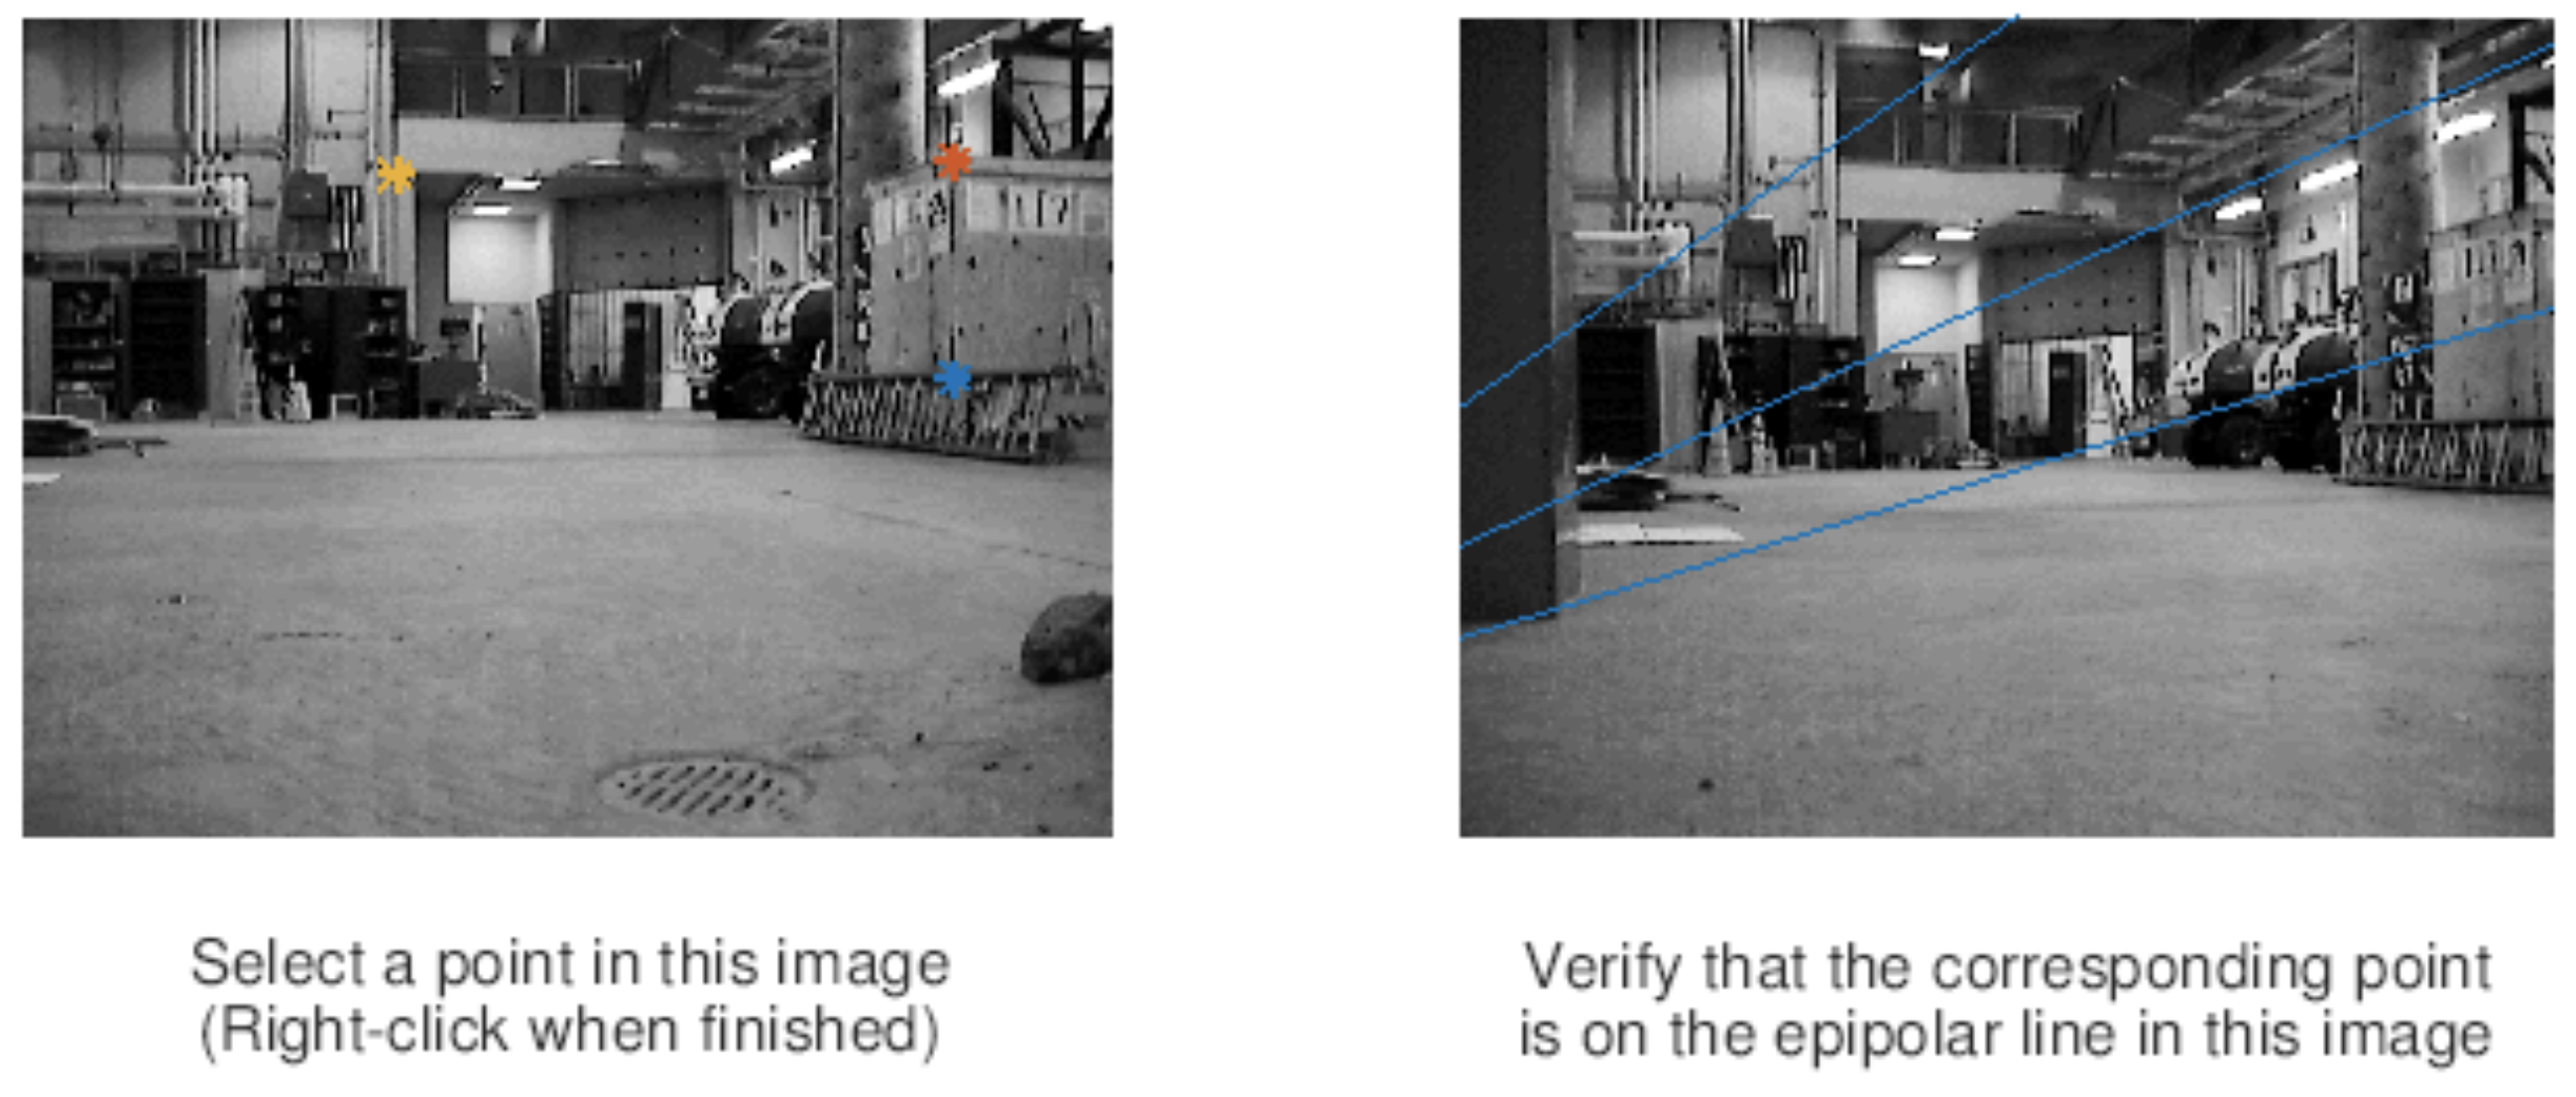
\includegraphics[width=0.85\linewidth]{1st_set_result.png}
                \caption{Epipolar lines found by $l_{r} = Fp_{l}$ ($1^{st}$ set)}
            \end{figure}
        For the second round, I think it will be better if I include more than 8 points. Hence, I concatenated the remaining two sets of data and computed the fundamental matrix again. The calculated fundamental matrix and testing result is shown in the figure below:
        \begin{equation}
            F _ {2} = \left[\begin{array} { ccc } { 4.6784 \mathrm { e } - 10 } & { - 9.2670 \mathrm { e } - 07 } & { 1.3625 \mathrm { e } - 04 } \\ { 7.0476 \mathrm { e } - 07 } & { 1.2601 \mathrm { e } - 07 } & {- 1.7650  \mathrm { e } - 03 } \\ { - 1.2534 \mathrm { e } - 04 } & { 1.7892 \mathrm { e } - 03} & { 4.5285 \mathrm { e } - 02 } \end{array}\right]
        \end{equation}
            \begin{figure}[H]
                \centering
                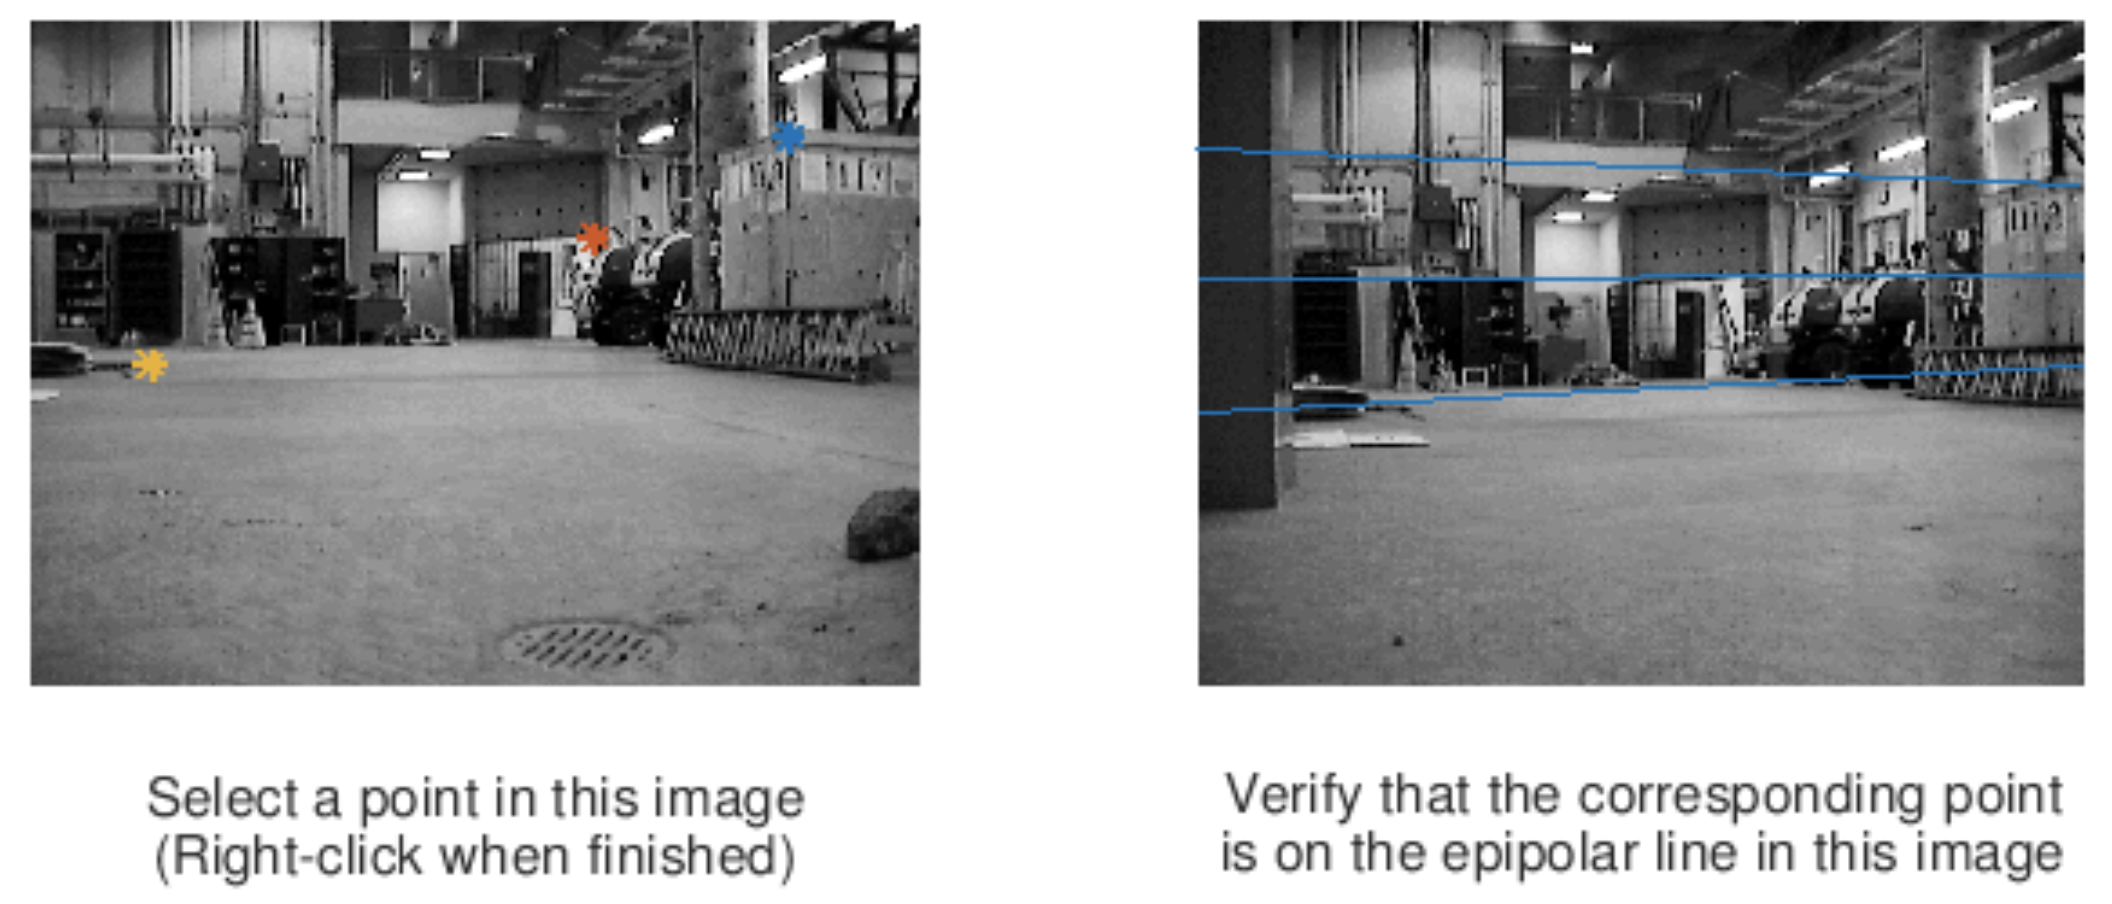
\includegraphics[width=0.85\linewidth]{23_set_result.png}
                \caption{Epipolar lines found by $l_{r} = Fp_{l}$ ($2^{nd}, 3^{rd} $ sets)}
            \end{figure}
        As shown, the results get much better than before in the sense that the corresponding epipolar lines go through the matched points. However, it is a bit strange that the position of the epipole now lies on the right of the second image.\\
        After these experiments, I think that the accuracy of the eight-point algorithm could be quite low if the matching points are not accurately selected. As pointed out in by Hartley \cite{defense}, the inaccuracies in the matching point measurement will result in $A$ not full rank. Consequently, we can only choose the least eigenvector of $A^{T}A$ to be our solution, and this introduce some errors. Although I used Harris feature detector to do the feature matching, there's still inaccuracy in the result. Besides the problem with matching points, this algorithm itself is also not very good. Instead, we can use some iterative algorithm like RANSAC to improve the results.
    \end{solution}
\end{subparts}

\part
\textbf{Final results and structured codes}\\
    To get more accurate results, I used Harris feature detector with more strict requirement and it outputs 17 points for me only. There are supposed to be best matched points and I used these data as input to calculate the fundamental matrix. My final result is shown below:

    \begin{equation}
        F = \left[ \begin{array} { r r r r } { - 3.9335 \mathrm { e } - 09 } & { 6.2600 \mathrm { e } - 07 } & { - 1.1718 \mathrm { e } - 04 } \\ { - 7.6470 \mathrm { e } - 07 } & { - 1.7108 \mathrm { e } - 08 } & { - 1.7488 \mathrm { e } - 03 } \\ { 1.5567 \mathrm { e } - 04 } & { 1.7997 \mathrm { e } - 03 } & { 4.5633 \mathrm { e } - 02 }  \end{array}\right]
    \end{equation}
    The Matlab source codes is attached together with this report, but for your convenience the complete codes for normalization and estimation are listed as follow:
            \begin{lstlisting}
I1 = imread('frc1.tif');
I2 = imread('frc2.tif');
% first computation
displayEpipolarF(I1,I2,estimateF(grp1a', grp1b'))   % transpose since the required input is 2 $\times$ n matrix

% second computation
displayEpipolarF(I1,I2,estimateF([grp2a; grp3a]', [grp2b; grp3b]'))

% final computation using better data omitted...

function [ normalized_pts, T_s ] = normalize( pts )
%   Input: points on an image
%   Output: normalized points for the use of eight_point_algo
    n = size(pts, 1);
    centroid = sum(pts, 1) / n;
    disp('The centroid is');
    disp(centroid);
    
    pts_demean = pts - centroid;
    
    squared_distance_sum = sum(sum(pts_demean.^2));
    
    scale_factor = sqrt(mean(squared_distance_sum) / 2);    % scale to sqrt(2)
    
    normalized_pts = pts_demean / scale_factor;
    
    disp('Check for the RMS average distance:');
    disp(sqrt(mean(sum(sum(normalized_pts.^2)))));
    
    % x' = s * (x + t_x) ; y' = s * (y + t_y)
    t_x = -centroid(1);
    t_y = -centroid(2);
    s = 1 / scale_factor;
    
    T_s = [s 0 s*t_x; 0 s s*t_y; 0 0 1];
    disp('The similarity transformation is');
    disp(T_s);
end


function F = estimateF(x1, x2)
    % x1 and x2 are each 2 x n matrices with the 
    % columns corresponding to the coordinates in the first
    % and the second image respectively
    pts1 = x1';
    pts2 = x2';
    
    [n_pts1, T_s1] = normalize(pts1);
    [n_pts2, T_s2] = normalize(pts2);
    
    % construct A
    A = [n_pts2(:,1).*n_pts1(:,1) n_pts2(:,1).*n_pts1(:,2) n_pts2(:,1) n_pts2(:,2).*n_pts1(:,1) n_pts2(:,2).*n_pts1(:,2) n_pts2(:,2) n_pts1(:,1) n_pts1(:,2) ones(size(n_pts1(:,1)))];
    % from svd(A), get F
    [U, S, V] = svd(A);
    F_temp = V(:,length(V));
    F_temp = reshape(F_temp, [3,3])';
    % enforce F singularity
    [U_f, S_f, V_f] = svd(F_temp);
    S_f(3,3) = 0;
    F_prime = U_f * S_f * V_f';
    
    %denormalization
    F = T_s2' * F_prime * T_s1;
end
        \end{lstlisting}
    
    \begin{figure}[H]
    \centering
    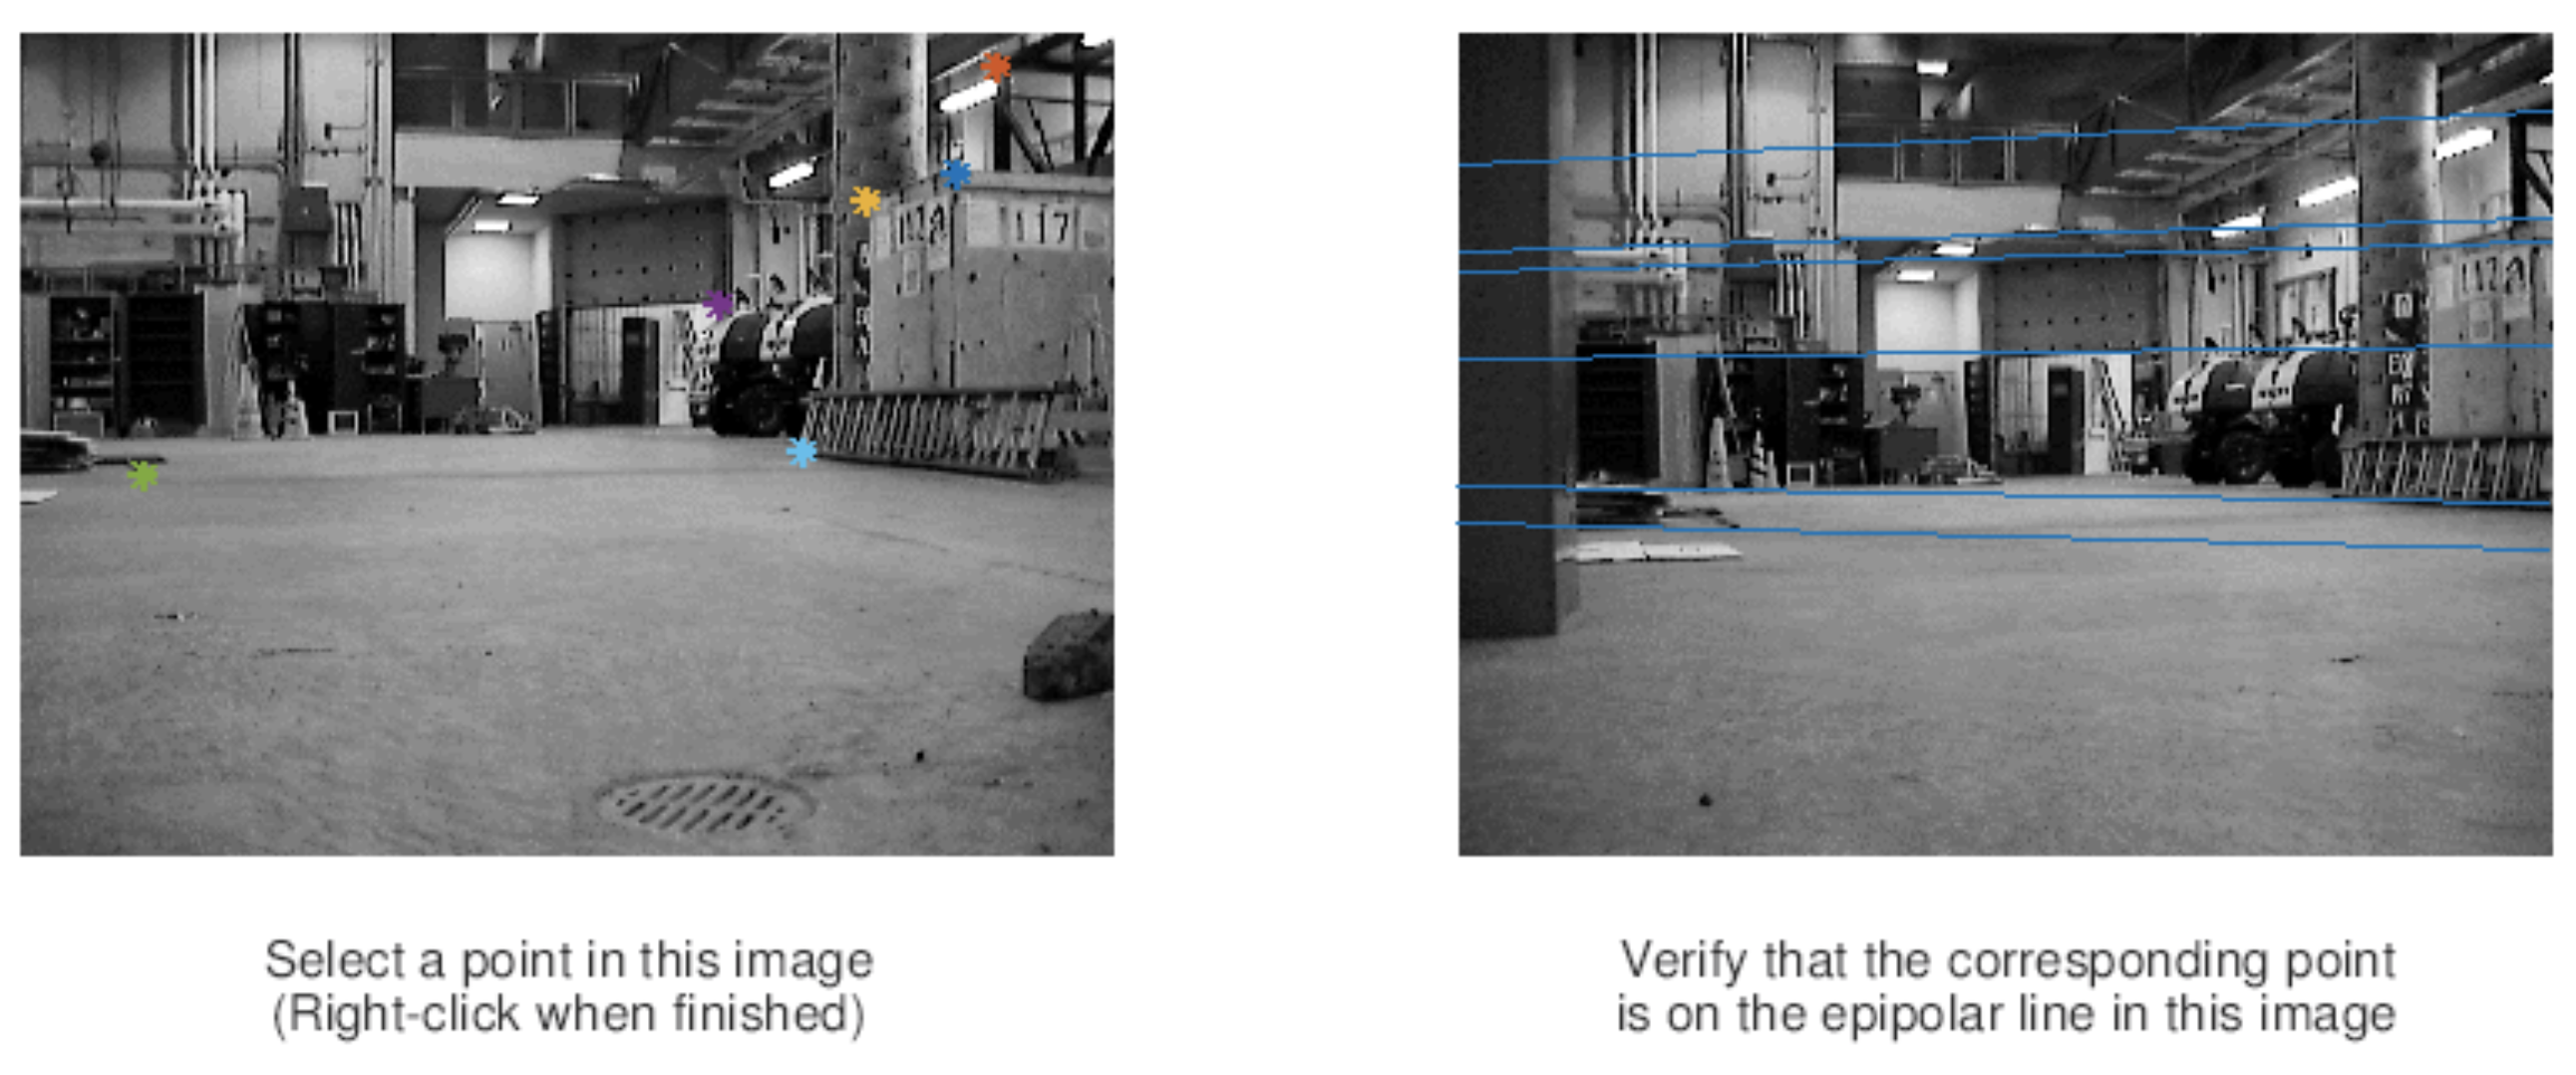
\includegraphics[width=0.85\linewidth]{visualize.png}
    \caption{Final (best) result}
    \end{figure}
    The figure above shows that for every point selected in the left image, the fundamental matrix can effectively find the corresponding epipolar line in the right image. This is obtained use the most accurate matched points I can get.
\end{parts}
\end{questions}
\clearpage

\section{Motion Perception}
\begin{questions}
\question
In the figure below, the two squares are translating horizontally in the opposite directions as indicated by the arrows. Indicate the respective perceived motions if you are looking through the apertures 1, 2, and 3. Explain your answers.

\begin{figure}[H]
    \centering
    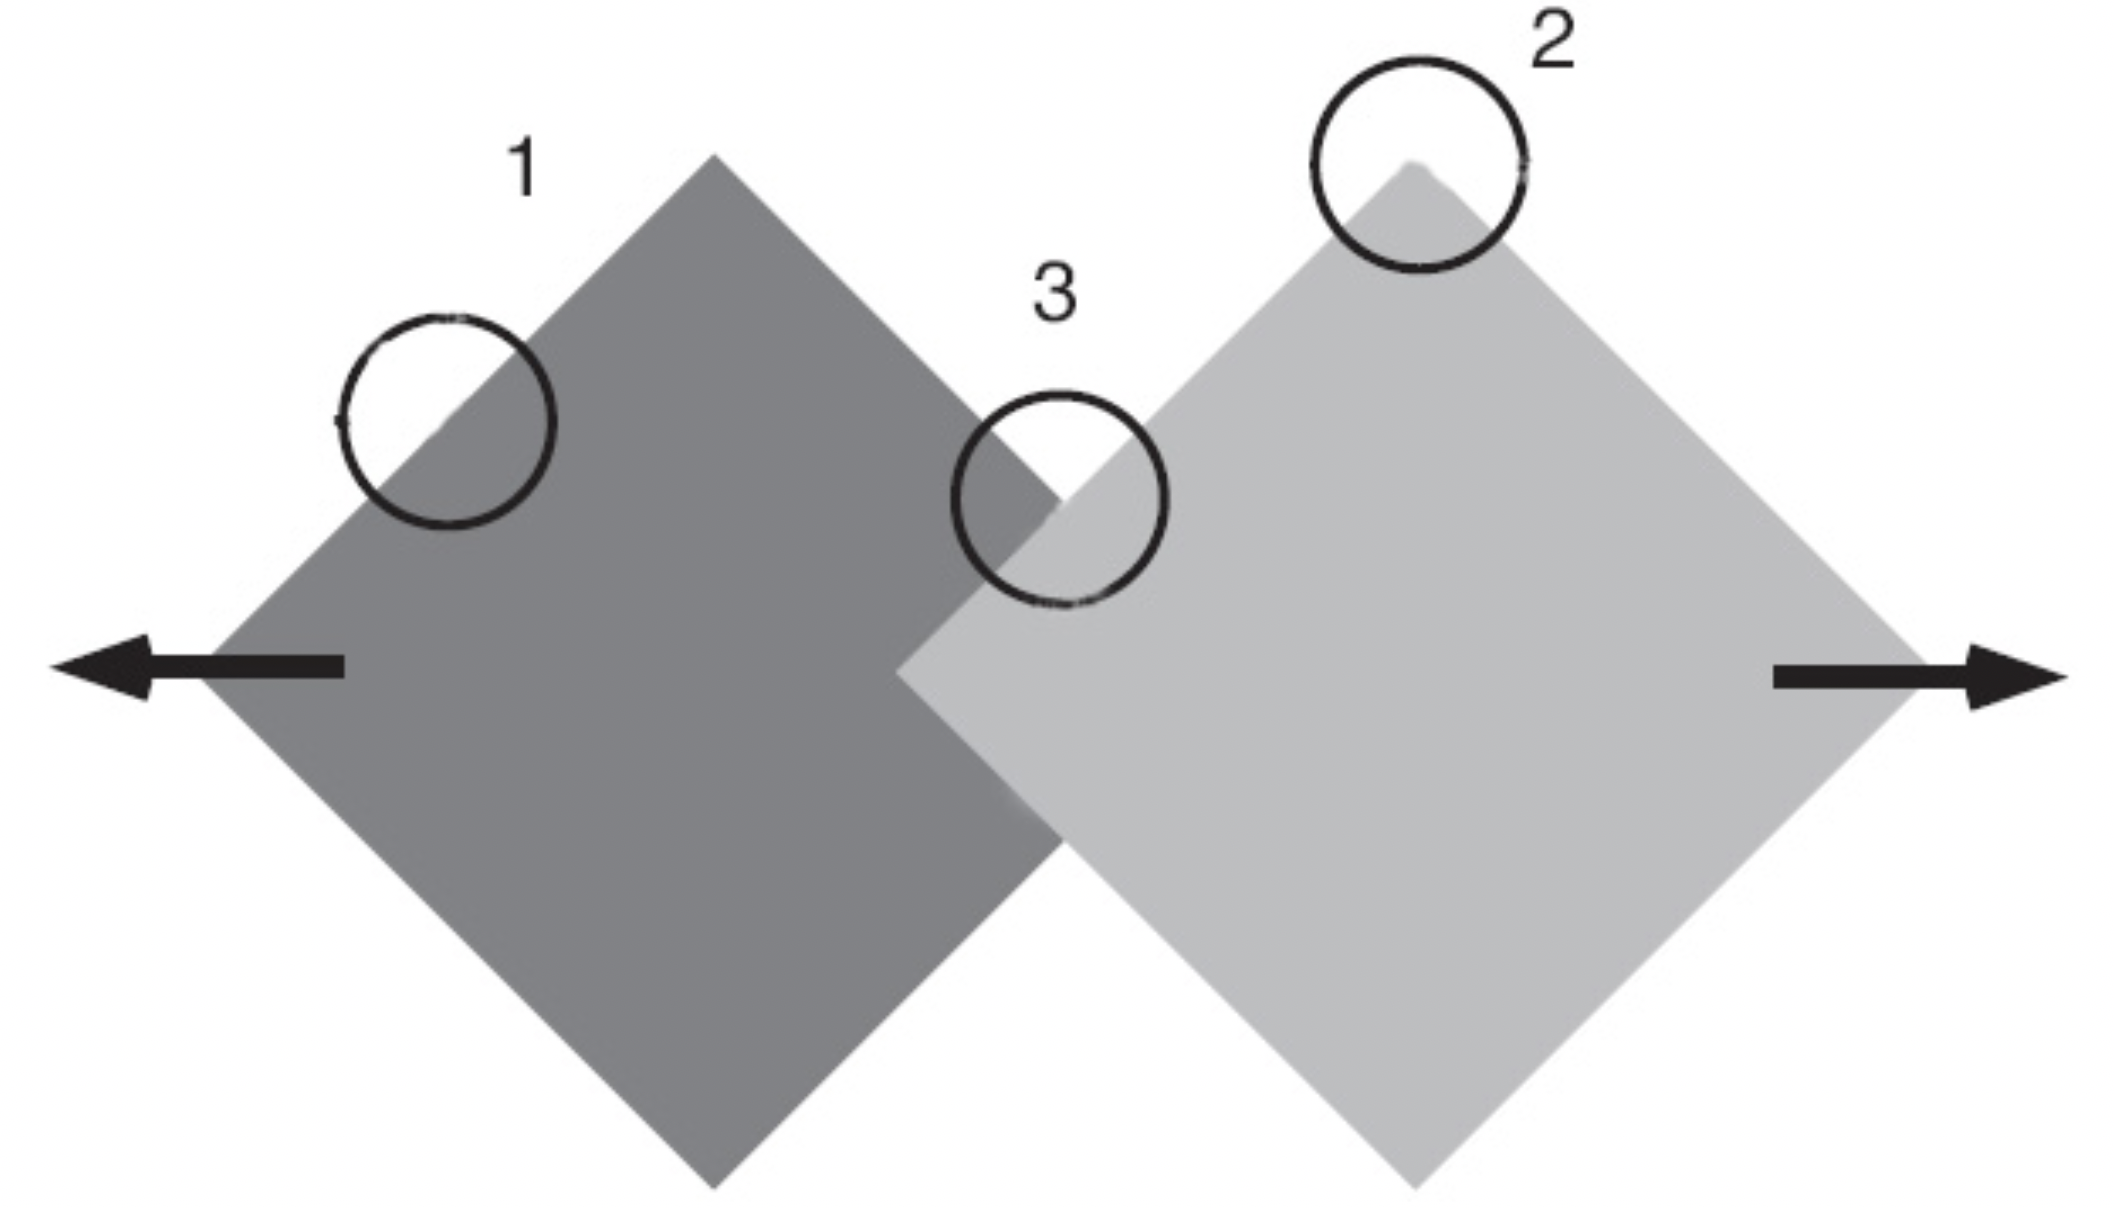
\includegraphics[width=0.6\linewidth]{square_motion.png}
    \caption{Two squares translating horizontally in the opposite directions.}
\end{figure}

\begin{solution}
    Based on Brightness Constancy Equation assumption, we humans can observe the normal flow of an object within an aperture.\\
    Donald Hoffman has explained this ``aperture problem" as the choice of our visual system to construct the smallest motion. This choice is motion orthogonal to the line that moves \cite{HD}.\\
    At \textbf{aperture 1}, the perceived motion will be pointing to the upper left direction that is perpendicular to the edge. This is because without context, we can only see the movement of the edge (the sharp change of intensity) and conclude that the object is moving perpendicular to its edge.\\
    At \textbf{aperture 2}, the perceived motion will be pointing vertically downwards, with the assumption that the two squares are moving with the same speed in the opposite direction. Due to symmetry, the corner formed by two edges of two squares will moving downwards. And because of it, we will perceive that the object is moving downwards since the corner is the motion clue we can see through this aperture.\\
    At \textbf{aperture 3}, the perceived motion will be pointing to the right. The reason is similar to aperture 2, with the corner giving us clues about the object's motion.
\end{solution}

\question
Barber-pole with Occlusion: The figure below illustrates various barber-pole configurations, with occluders placed along either vertical or horizontal sides of the barber-pole. The arrows indicate the perceived direction of barber-pole motion. Explain why the perceived motion tends to be biased in the direction orthogonal to the occlusion boundary.

\begin{figure}[H]
    \centering
    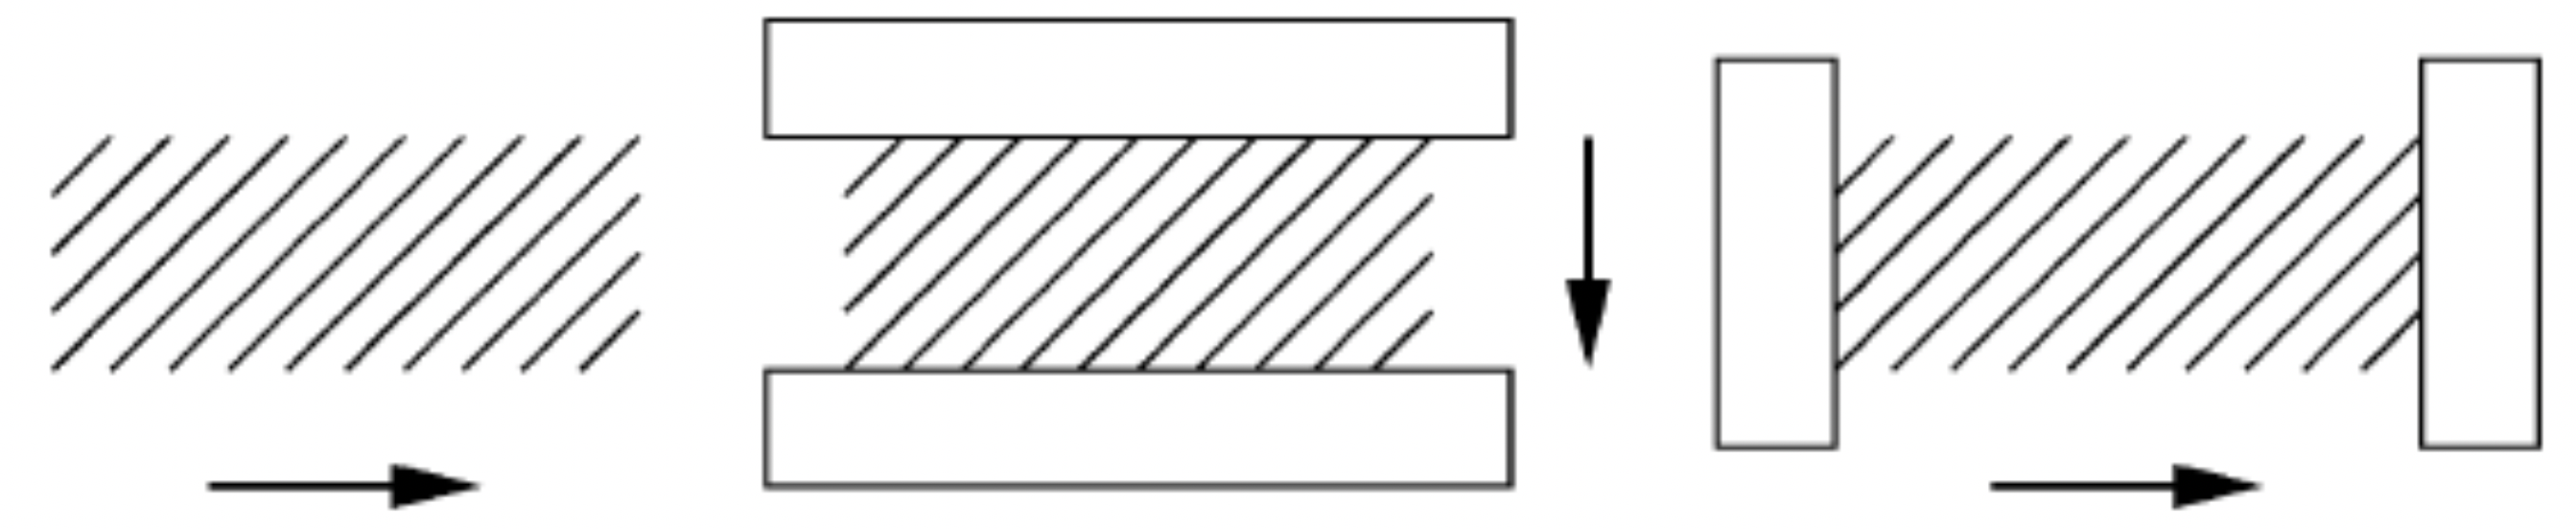
\includegraphics[width=0.6\linewidth]{Barber_pole.png}
    \caption{Barber-pole with occlusion. Arrows indicate the perceived motion. Left: Barber-pole with no occluders. Middle: Occluders placed on the top and bottom cause the perceived motion to be mostly vertical. Right: Occluders placed on the left and right sides of the barber-pole bias the perceived motion toward horizontal.}
\end{figure}

\begin{solution}
    For a barber-pole, the diagonally oriented lines are spinning inside the occluder. However, he eyes use the visual cues where the stripes end at the sides of the pole to override any visual depth cues, and therefore the stripes appear to move vertically or horizontally rather than spin. \\
    In addition, the line terminators aligned with the occluders are considered as \textbf{extrinsic} terminators, therefore their motion signals tend to
    become more ambiguous and have less influence on the perceived motion \cite{vis04}. This is the reason for perceiving the middle scenario as moving downwards. And for the right scenario, it is obvious that more number of intrinsic terminators are moving horizontally so that we perceive it moving rightwards. 
\end{solution}

\question
* Referring to the diagram below, the stimulus consists of two orthogonal bars that move sinusoidally, 90 degree out of phase (Figure a and b). When presented together within an occluding aperture (Figure c), the bars perceptually cohere and appear to move in a circle as a solid cross. However, when presented alone (Figure d), they appear to move separately (the horizontal bar translates vertically and the vertical bar translates horizontally), even though the image motion is unchanged in Figures c and d. In either stimulus condition, both percepts are legitimate interpretations of the image motion. Yet a single interpretation is predominantly seen in each case. Why?

\begin{figure}[H]
    \centering
    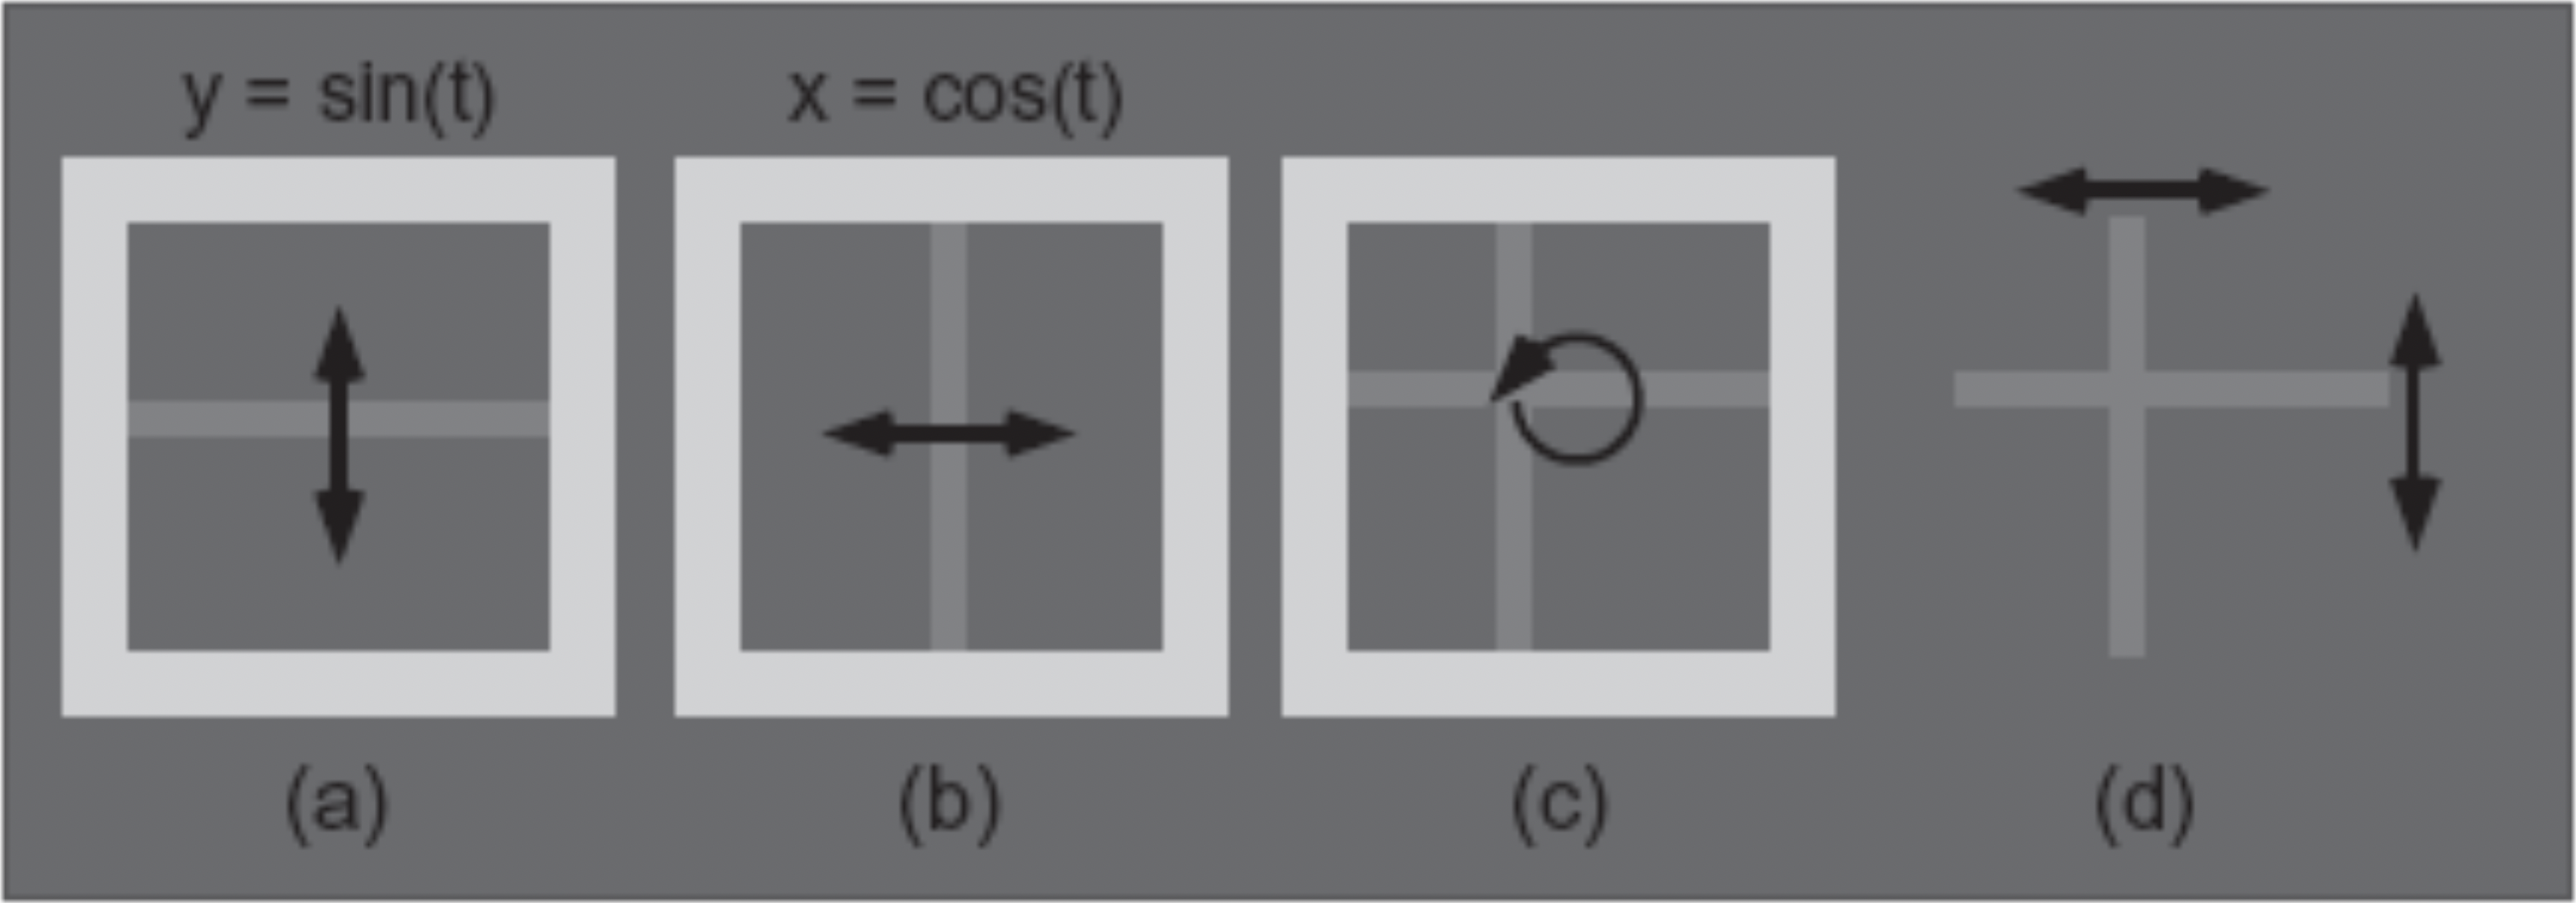
\includegraphics[width=0.6\linewidth]{stimulus.png}
\end{figure}

\begin{solution}
    In the configuration (d), the bar endpoints are clearly seen by viewers. It can provide unambiguous two dimensional motion signals, which are believed to determine the motion percept. The endpoints move linearly, and each bar follows along.\\
    However, when the frame is present, the T-junctions are formed at the bar endpoints. These junctions provide a cue that the endpoint motions are the spurious result of occlusion. Thus, the motion at T-junctions will have less influence on our perception. With this, the circular motion of the bar intersection determines the motion percept, as all the local motions in the stimulus apart from those of the endpoints are consistent with such a circular motion.
\end{solution}

\question
* For a purely rotational motion, the equation that relates the optical flow $(u, v)$ to its rotational parameters $(\omega_{x}, \omega_{y}, \omega_{z})$ is of the conic form explored in Questions $3d$ and $3e$:
\begin{equation}
        \begin{aligned} u &=\omega_{x} x y-\omega_{y}\left(x^{2}+1\right)+\omega_{z} y \\ v &=\omega_{x}\left(y^{2}+1\right)-\omega_{y} x y-\omega_{z} x \end{aligned}
\end{equation}
Assume you are given enough optical flow measurements at different $(x, y)$ locations, solve $(\omega _ {x}, \omega _ {y}, \omega _ {z})$ in the least squares sense by writing down the least squares equation of the form $Ax=b, (b \neq 0)$. Explain why in this case, the equation is of the non-homogeneous form, whereas that in Question 3e is of the homogeneous form $Ax=0$, and explain whether it is appropriate or inappropriate to change the formulation of this question to the $Ax=0$ form.

\begin{solution}
    The least squares equation is formed as:
    \begin{equation}
        \begin{bmatrix}
            xy & -(x^{2} + 1) & y \\
            y ^ {2} + 1 & -xy & -x
        \end{bmatrix}
        \left( \begin{array}{c}
           \omega _ {x} \\  
           \omega _ {y} \\  
           \omega _ {z} \\  
        \end{array}\right) = \left(\begin{array}{c}
             u \\
             v
        \end{array}\right)
    \end{equation}
    In this question, there are three unknowns and two equations. The matrix is rank-deficient and thus we'd like to use SVD and compute the psedo-inverse. It is not suitable to change to $Ax=0$ (homogeneous) form because the null vector will not be unique. But in question 3e, which is an over-determined question, we just take the eigenvector of $A^{T}A$ corresponding to the smallest singular value.
    
\end{solution}
    


\end{questions}
    





\clearpage

\bibliographystyle{siam}
\bibliography{bibliography.bib}
\end{document}